\chapter{Results}
\label{chapter 6}
\ifpdf
    \graphicspath{{Chapter6/Figs/}{Chapter6/Figs/PDF/}{Chapter6/Figs/}}
\else
    \graphicspath{{Chapter6/Figs/Vector/}{Chapter6/Figs/}}
\fi
This chapter aims to present a general, yet as much as possible complete collection of KPI behaviors, showing the most meaningful simulation results. Each KPI is plotted to display its behavior when a variation occurs. The graphs present all the same structure, showing the KPI values as a function of the job IDs (i.e. Case IDs). \\
For the sake of brevity, Basic KPIs plots are not discussed: the analysis would be too lengthy and dispersive, and they would be difficult to visualize since the data noise makes them barely understandable. Therefore, only RW KPIs are considered, with parameters $f = 100$ and $l = 100$. Moreover, in Processing\_time plots and CCI plots, the average inter-arrival time is displayed with a dashed line in correspondence with the value $\mu_a=10$.
\section{Processing time variation}
A processing time variation not only causes a change in Processing\_time basic and derived KPIs in correspondence with the changing stage, but also influences different KPIs in all other stages, upstream and downstream the changing stage. \\
In this section the most information-rich indicators are analyzed, starting from consecutive case intervals KPIs and their relationship with cycle time. Then, it is shown how processing time variations are directly displayed by Processing\_time. After that, the complex behavior of Blocking\_time and Starving\_time is described. Lastly, Waiting\_time and its suitability to show variations in queue lengths are presented.
\newpage
\subsection{Consecutive cases intervals KPIs}
\label{Consecutive cases intervals KPIs - Processing time variation}
Consecutive cases intervals (CCI) KPIs are indicators strongly related to the cycle time. First of all, the behavior of one of them, Mid\_diff, is shown in a processing time increase situation. Then, the stage synchronization caused by the cycle time propagation through the line is displayed with this KPI. Finally, it is shown how similar are the behaviors of Input\_diff and Output\_diff with respect to Mid\_diff.
\subsubsection{Processing time increase effects on Mid\_diff}
\begin{figure}[h] 
\centering
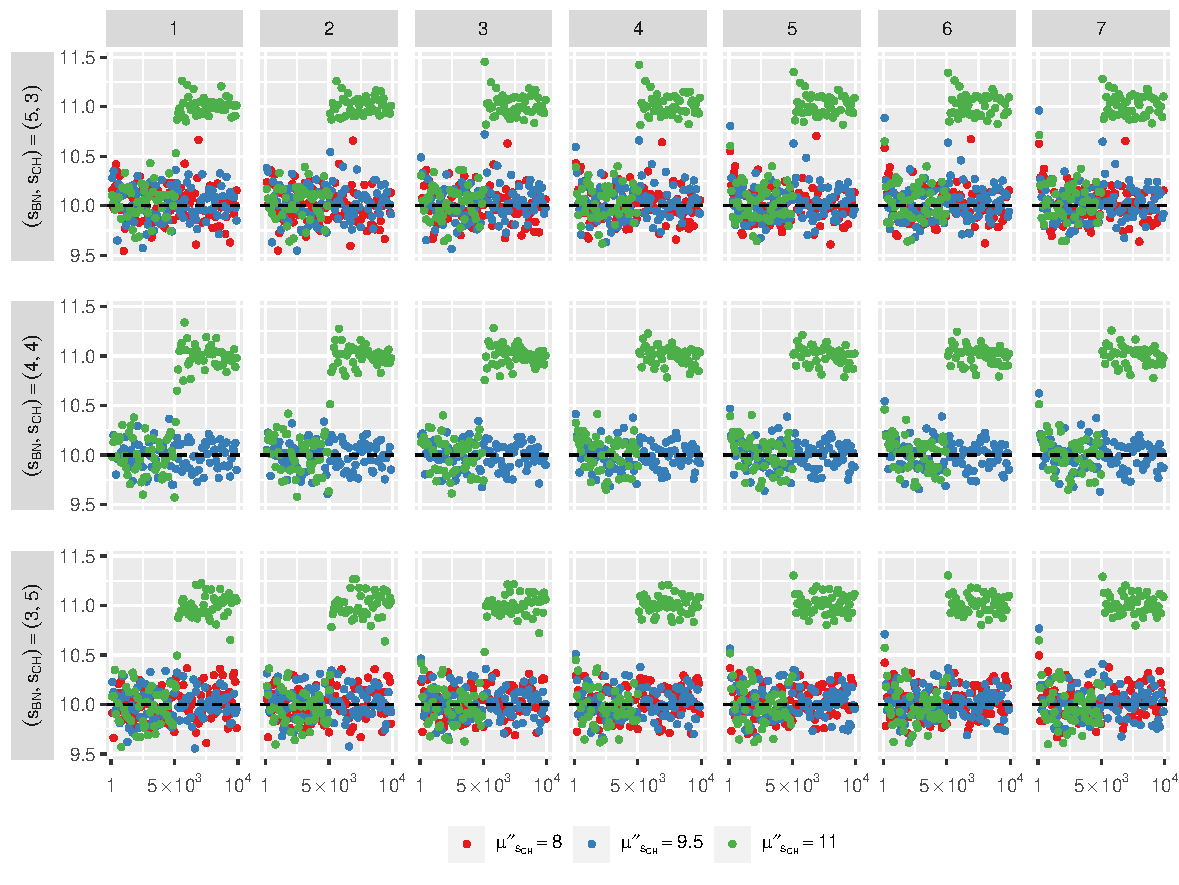
\includegraphics[width=1\textwidth]{ProcessingIncrease1_Mid_diff_MEAN}
\caption[Mid diff RW KPI behavior considering different processing time increase levels]{Mid diff RW KPI considering three mean processing time increase levels $\mu_{s_{CH}}''$ and three bottleneck - changing stage configurations $(s_{BN},s_{CH})$. Models with $cl_s=6$.}
\label{fig:Mid diff RW KPI behavior with different processing time increase levels}
\end{figure}
Figure \ref{fig:Mid diff RW KPI behavior with different processing time increase levels} shows Mid\_diff\_MEAN RW KPI behavior when a processing time growth occurs. It can be deduced that
\begin{itemize}
\item Before the variation, the system is stable and average Mid\_diff stabilizes around the average inter-arrival time $\mu_a$. \\This is visible in all the models until Case ID reaches value $5000$.
\item If a resource loses capacity, but the system remains stable (i.e. $\mu_{s_{CH}}''<\mu_a$) average Mid\_diff does not change and remains around the average inter-arrival time $\mu_a$. \\This is visible in models with $\mu_{s_{CH}}''=8$ and $\mu_{s_{CH}}''=9.5$ after Case ID has reached value $5000$.
\item If a resource loses capacity to the point that the system becomes unstable (i.e. $\mu_{s_{CH}}''>\mu_a$), average Mid\_diff increases and aligns with the bottleneck average processing time $\mu_{s_{CH}}''$. \\This is visible in model with $\mu_{s_{CH}}''=11$ after Case ID has reached value $5000$.
\item The value taken by average Mid\_diff does not depend on the stage position with respect to the changing stage $s_{CH}$ or the bottleneck $s_{BN}$: it behaves similarly in all stages. \\This is visible comparing models having different bottleneck-changing stage configurations $(s_{BN},s_{CH})$.
\end{itemize}
Mid\_diff follows the cycle time behavior as it is described in theory: it stands around a value equal to the maximum between the bottleneck average processing time $\mu_{s_{BN}}$ and the average inter-arrival time $\mu_a$\footnote{Actually, the average cycle time is equal to the maximum between the average inter-arrival time, average bottleneck processing time and average inter-departure time from the last stage, but since job departures from the system are assumed unconstrained in this thesis, the last term can be omitted.}. 
\subsubsection{Mid\_diff propagation along the line}
Even if it is scarcely visible in figure \ref{fig:Mid diff RW KPI behavior with different processing time increase levels}, Mid\_diff does not immediately change in all stages, exactly like system cycle time: when the system becomes unstable, the new cycle time needs a certain time span to spread in stages both upstream, through blocking, and downstream, through starvation. Time required to re-establish process synchronization across the line depends mainly on current saturation of buffers: the more the buffers upstream are unsaturated, the longer cycle time takes to propagate upstream (blocking is delayed). The opposite occurs for downstream stages, where cycle time spread is slower the more the buffers are saturated (starvation is delayed). 
\begin{figure}[h] 
\centering
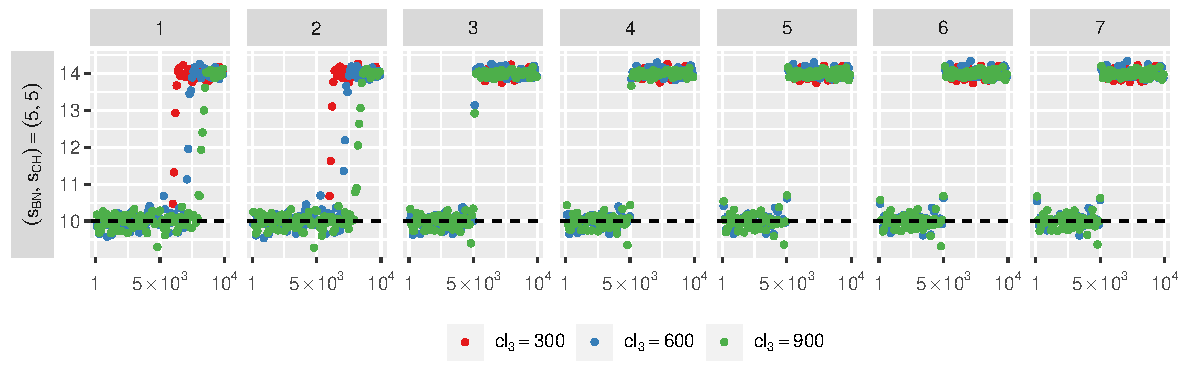
\includegraphics[width=1\textwidth]{ProcessingIncrease2_Mid_diff_MEAN}
\caption[Mid diff RW KPI variation delays considering different buffer capacity limits]{Mid diff RW KPI variation delays in case of a mean processing time increase $\mu_{s_{CH}}''$ considering different buffer capacity limits $cl_3$. Models with configuration $(s_{BN},s_{CH})=(5,3)$ and processing time increase $\mu_{s_{CH}}''=14$.}
\label{fig:Mid diff RW KPI variation delays considering different buffer capacity limits}
\end{figure}
Figure \ref{fig:Mid diff RW KPI variation delays considering different buffer capacity limits} better displays what just explained: the graphs portray a particular system where a single buffer having high capacity limit, placed in stage $s=3$, is extremely unsaturated before the variation occurs. After the first stage has processed $5000$ jobs, the resource in the bottleneck stage $s=5$, positioned downstream stage $s=3$, looses production capacity and its processing time increases to the point that it exceeds inter-arrival time and the system becomes unstable. Therefore cycle time increases, aligning with the new bottleneck average processing time, but the high capacity buffer works as a temporary decoupling point, delaying the blocking and, so, the synchronization of stages upstream its position. Moreover, these plots show that the bigger the buffer capacity ($cl_3$), the wider is the time span before cycle time (i.e. Mid\_diff) manages to spread upstream that stage.\\
This means that, a variation that has effects on CCI KPIs is immediately detectable only in correspondence of the changing stage, while in the rest of the stages the variation could be delayed due to low (or high, when cycle time spreads downstream) buffer saturation levels. 
\subsubsection{Input\_diff and Output\_diff behaviors}
\begin{figure}[h] 
\centering
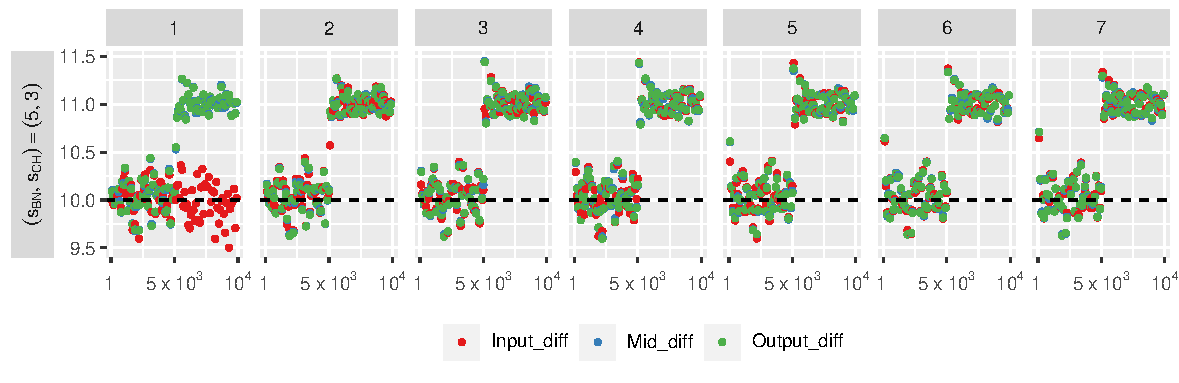
\includegraphics[width=1\textwidth]{ProcessingIncrease3_Input_diff_MEAN_Mid_diff_MEAN_Output_diff_MEAN}
\caption[Different CCI RW KPIs behaviors compared]{Different CCI RW KPIs behaviors compared . Models with configuration $(s_{BN},s_{CH})=(4,4)$, $cl_s=6$, and $\mu_{s_{CH}}''=11$.}
\label{fig:Different CCI RW KPIs behaviors compared}
\end{figure}
Input\_diff and Output\_diff behave similarly to Mid\_diff, as figure \ref{fig:Different CCI RW KPIs behaviors compared} shows. Sure enough, CCI KPIs are all indicators of cycle time as it is seen in different stage positions. However, these KPIs are not exactly equal, and Input\_diff and Mid\_diff are not interchangeable when it comes to compute Starving time and Stage State RW KPIs: since Input\_diff is relative to buffer entrances, it becomes equal to Mid\_diff, which instead is relative to buffer exits, only when the buffer is saturated and the previous resource starts to suffer of blocking. So, in general, it cannot be used to calculate the exact Starving\_time and cannot serve as denominator in Utilization, Blocking\_prob and Starving\_prob.\\
Therefore, values taken by CCI KPIs are very similar, but they differ from each other for little delays in their behaviors and generally are not exactly equal.
\subsubsection{Input\_diff in the first stage}
Since the production lines considered in this thesis always have an unlimited buffer in the first stage, Input\_diff allows to know the average inter-arrival time even when the system becomes unstable. As a matter of fact, the first buffer completely isolates the line entrance from potential system instabilities, and so Input\_diff of the first stage is actually a permanent indicator of inter-arrival time, rather than an indicator of cycle time. This detail is visible in the the first stage plot of figure \ref{fig:Different CCI RW KPIs behaviors compared}: after the variation, Mid\_diff and Output\_diff increase, while Input\_diff does not change and remains equal to the average arrival time.
\newpage
\subsection{Processing\_time and Utilization KPIs}
\label{Processing time and Utilization KPIs - Processing time variation}
Processing\_time is the most useful indicator to understand if a resource production capacity has changed and to determine its new value. In this subsection, Processing\_time behavior is analyzed in situations of processing time increase and decrease. Then, Utilization KPI is presented and its relation with Processing\_time is displayed. 
\subsubsection{Processing time increase effects on Processing\_time KPI}
\begin{figure}[h] 
\centering
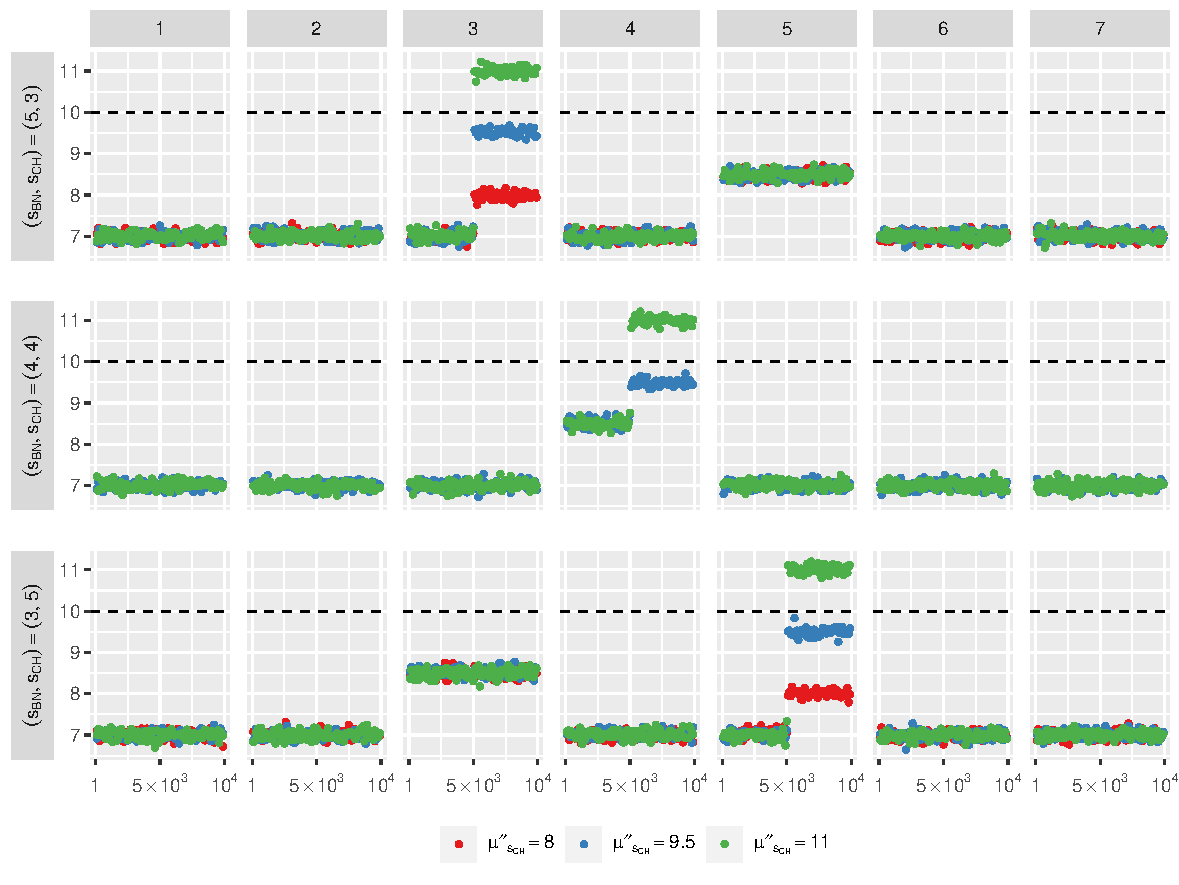
\includegraphics[width=1\textwidth]{ProcessingIncrease4_Processing_time_MEAN}
\caption[Processing time RW KPI behavior considering different processing time increase levels]{Processing time RW KPI behavior considering three mean processing time increase levels $\mu_{s_{CH}}''$ and three bottleneck - changing stage configurations $(s_{BN},s_{CH})$. Models with $cl_s=6$.}
\label{fig:Processing time RW KPI behavior with different processing time increase levels}
\end{figure}
Figure \ref{fig:Processing time RW KPI behavior with different processing time increase levels} shows Processing\_time\_MEAN RW KPI behavior when the production capacity of a stage reduces. 
\begin{itemize}
\item If a resource loses production capacity, average Processing\_time of the changing stage grows, while average Processing\_time of all other stages does not change. \\This is visible comparing the behavior of Processing\_time in correspondence with stage the changing $s_{CH}$ (where it increases) with its behavior in other stages (where it does not change). 
\item If a resource loses production capacity, the variation of changing stage average Processing\_time is such that the KPI value settles around the new average processing time of the stage. \\This is visible in each changing stage $s_{CH}$ plot. 
\item Average Processing\_time variation does not depend on the stage position with respect to the changing stage $s_{CH}$ or the bottleneck $s_{BN}$. \\This is visible comparing average Processing\_time behavior in the three different bottleneck - changing stage configurations $(s_{BN},s_{CH})$. 
\item Average Processing\_time variation does not depend on the system stability. \\This is visible comparing average Processing\_time behavior in models with $\mu_{s_{CH}}''=8$ and $\mu_{s_{CH}}''=9.5$ (where the system remains stable) with its behavior in model with $\mu_{s_{CH}}''=11$ (where the system becomes unstable).
\item Average Processing\_time of stage $s$ always stabilizes around the average time needed by stage $s$ resource to process a job. \\This is visible in all models, before and after the variation occurring when Case ID reaches value $5000$.
\end{itemize}
To summarize, the graphs show that the average Processing\_time of a stage is constantly aligned with the average processing time of that stage, even when the stage production capacity decreases. 
\subsubsection{Processing time decrease effects on Processing\_time KPI}
\begin{figure}[h] 
\centering
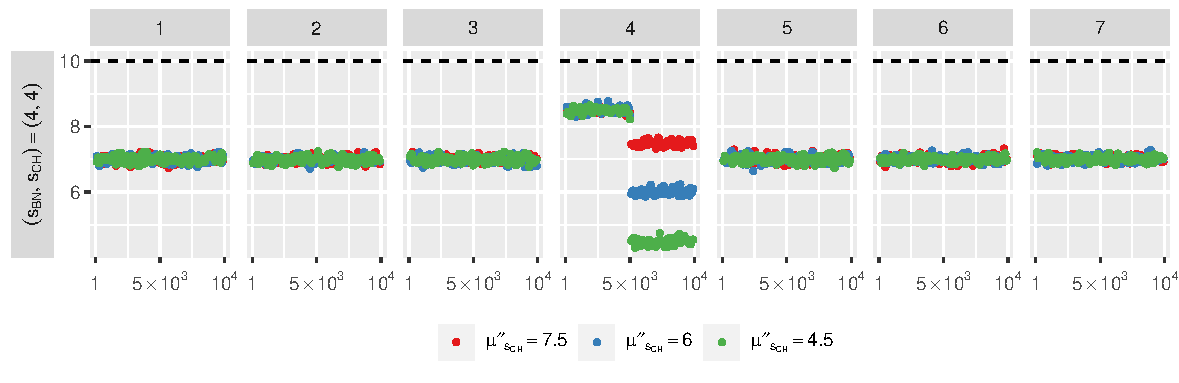
\includegraphics[width=1\textwidth]{ProcessingIncrease5_Processing_time_MEAN}
\caption[Processing time RW KPI behavior with different processing time decrease levels]{Processing time RW KPI behavior considering three different mean processing time decrease levels $\mu_{s_{CH}}$. Models with configuration $(s_{BN},s_{CH})=(4,4)$, and $cl_s=6$.}
\label{fig:Processing time RW KPI behavior with different processing time decrease levels}
\end{figure}
Figure \ref{fig:Processing time RW KPI behavior with different processing time decrease levels} shows Processing\_time\_MEAN RW KPI behavior when the production capacity of a stage increases. Looking at these plots it can be concluded that the observations made on average Processing\_time behavior in case of production capacity decrease can be extended to production capacity variations in general. Indeed, the only difference with the production capacity decrease case is that average Processing\_time of the changing stage $s_{CH}$ reduces when production capacity increases to keep aligned with the average processing time of that stage.
\subsubsection{Utilization KPI}
Processing\_time alone is useful to monitor stage production capacities, but does not give insights about how much stages work with respect to the line throughput. To obtain this information, Processing\_time\_MEAN with Mid\_diff\_MEAN are combined to calculate Utilization KPI.
\begin{figure}[h] 
\centering
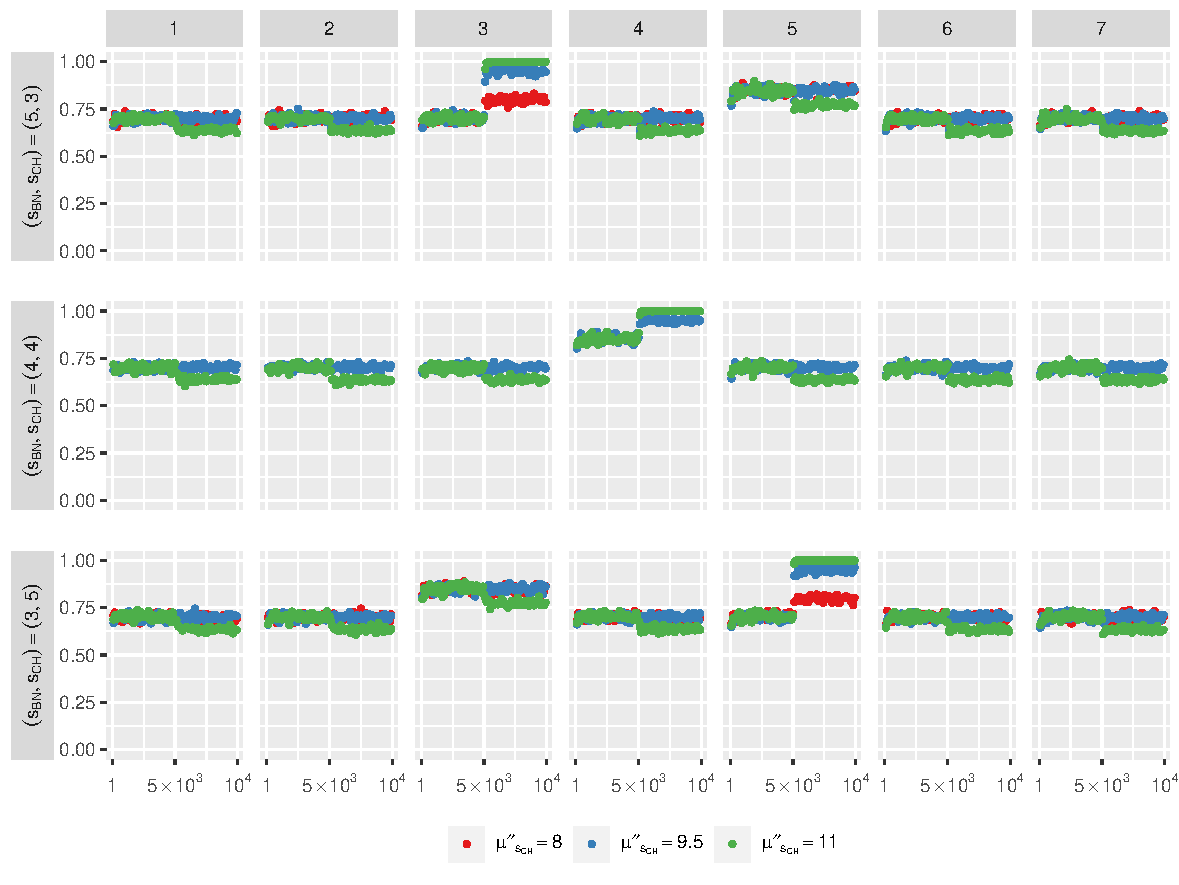
\includegraphics[width=1\textwidth]{ProcessingIncrease6_Utilization}
\caption[Utilization KPI behavior with different processing time increase levels]{Utilization KPI behavior considering three mean processing time increase levels $\mu_{s_{CH}}''$ and three bottleneck - changing stage configurations $(s_{BN},s_{CH})$. Models with $cl_s=6$.}
\label{fig:Utilization KPI behavior with different processing time increase levels}
\end{figure}
Figure \ref{fig:Utilization KPI behavior with different processing time increase levels} shows Utilization KPI behavior when the production capacity of a stage reduces. This KPI behavior is similar to average Processing\_time behavior, with some important differences
\begin{itemize}
\item If a resource loses production capacity, but the system remains stable, Utilization of the changing stage grows, while Utilization of all other stages does not change. \\This is visible in models with $\mu_{s_{CH}}''=8$ and $\mu_{s_{CH}}''=9.5$, comparing the behavior of Utilization in correspondence with stage the changing $s_{CH}$ (where it increases) with its behavior in other stages (where it does not change). 
\item If a resource loses production capacity to the point that the system becomes unstable, Utilization of the changing stage grows and settles to value $1$, while Utilization of all other stages reduces. \\This is visible in models with $\mu_{s_{CH}}''=11$, comparing the behavior of Utilization in correspondence with stage the changing $s_{CH}$ (where it increases) with its behavior in other stages (where it decreases). 
\item Utilization variation does not depend on the stage position with respect to the changing stage $s_{CH}$ or the bottleneck $s_{BN}$. This is visible comparing Utilization behavior in the three different bottleneck - changing stage configurations $(s_{BN},s_{CH})$. 
\item Values taken by Utilization are limited to the range $[0,1]$. \\This is visible in all models, before and after the variation occurring when Case ID reaches value $5000$.
\item Utilization of stage $s$ stabilizes around the average utilization of stage $s$ resource. \\This is visible in all models, before and after the variation occurring when Case ID reaches value $5000$.
\end{itemize}
Utilization KPI follows the theoretical behavior of resource utilization. Indeed, the utilization of a resource is equal to the ratio between throughput and production capacity of the resource, or in other words, it is equal to the ratio between the resource processing time and the system cycle time. Therefore, if the system becomes unstable, cycle time grows aligning with the bottleneck processing time, and so the resource utilization in the bottleneck reaches $100\%$. Instead, after all other stages have synchronized with the bottleneck lowering their throughput, their utilization reduces.\\
Even if the relative plots are not shown, it is possible to extend the observations made on Utilization behavior in case of production capacity decrease to production capacity variations in general, as with average Processing\_time. The only difference with the production capacity decrease case is that Utilization of the changing stage $s_{CH}$ reduces when production capacity increases to keep always aligned with utilization of that stage.
\newpage
\subsection{Blocking\_time, Starving\_time and respective Stage State KPIs}
\label{Blocking time, Starving time and respective Stage State KPIs - Processing time variation}
Blocking\_time and Starving\_time KPIs are analyzed together because of their strong relationship. As a matter of fact, their behavior is specular, since they both depend on the resource utilizations and on the buffer capacities. This subsection starts showing and discussing these KPI general behaviors and the effects of a processing time variation on them. Then, Bloking\_prob and Starving\_prob, which are respectively Blocking\_time and Starving\_time derived Stage State KPIs, are commented. 
\subsubsection{Processing time increase and reduction effects on Blocking\_time and Starving\_time KPIs}
\begin{figure}[h] 
\centering
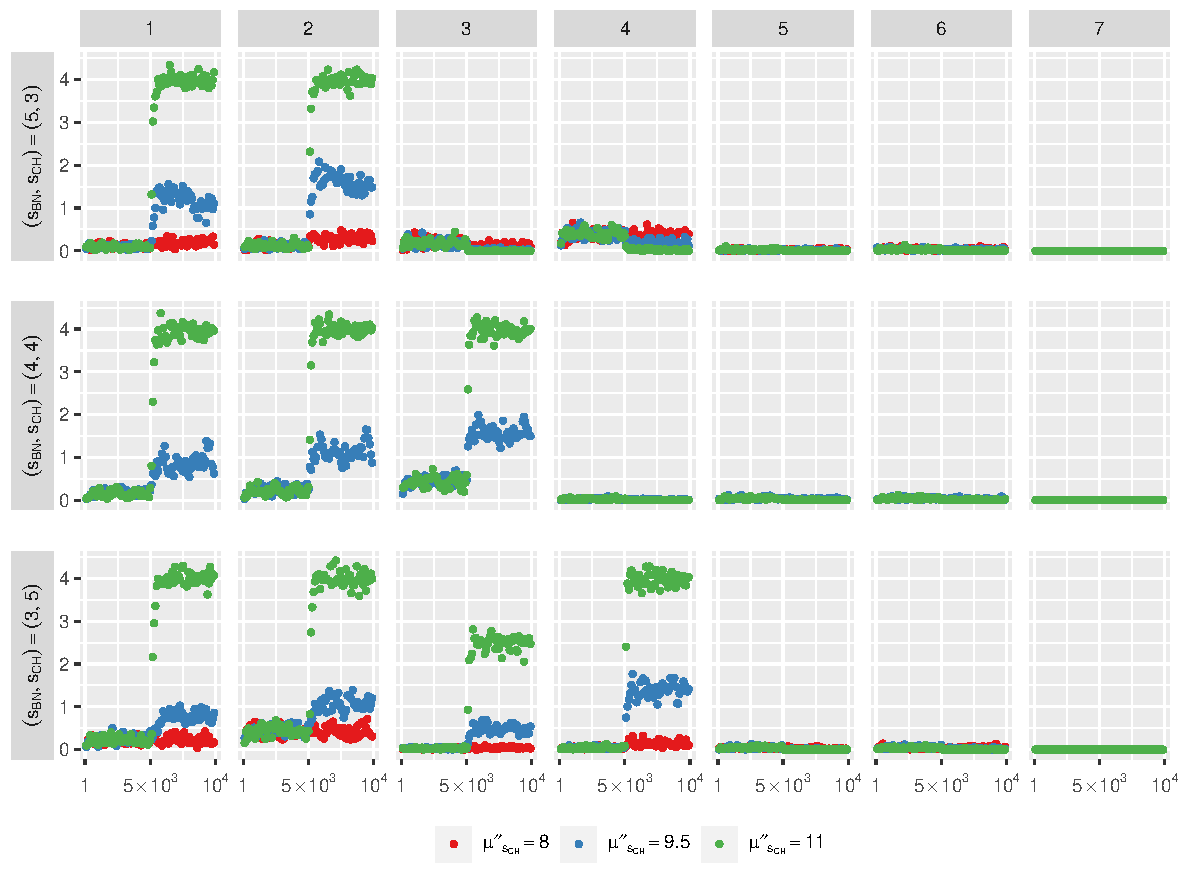
\includegraphics[width=1\textwidth]{ProcessingIncrease7_Blocking_time_MEAN}
\caption[Blocking time RW KPI behavior with different processing time increase levels]{Blocking time RW KPI considering three mean processing time increase levels $\mu_{s_{CH}}''$ and three bottleneck - changing stage configurations $(s_{BN},s_{CH})$. Models with $cl_s=6$.}
\label{fig:Blocking time RW KPI behavior with different processing time increase levels}
\end{figure}
\begin{figure}[h] 
\centering
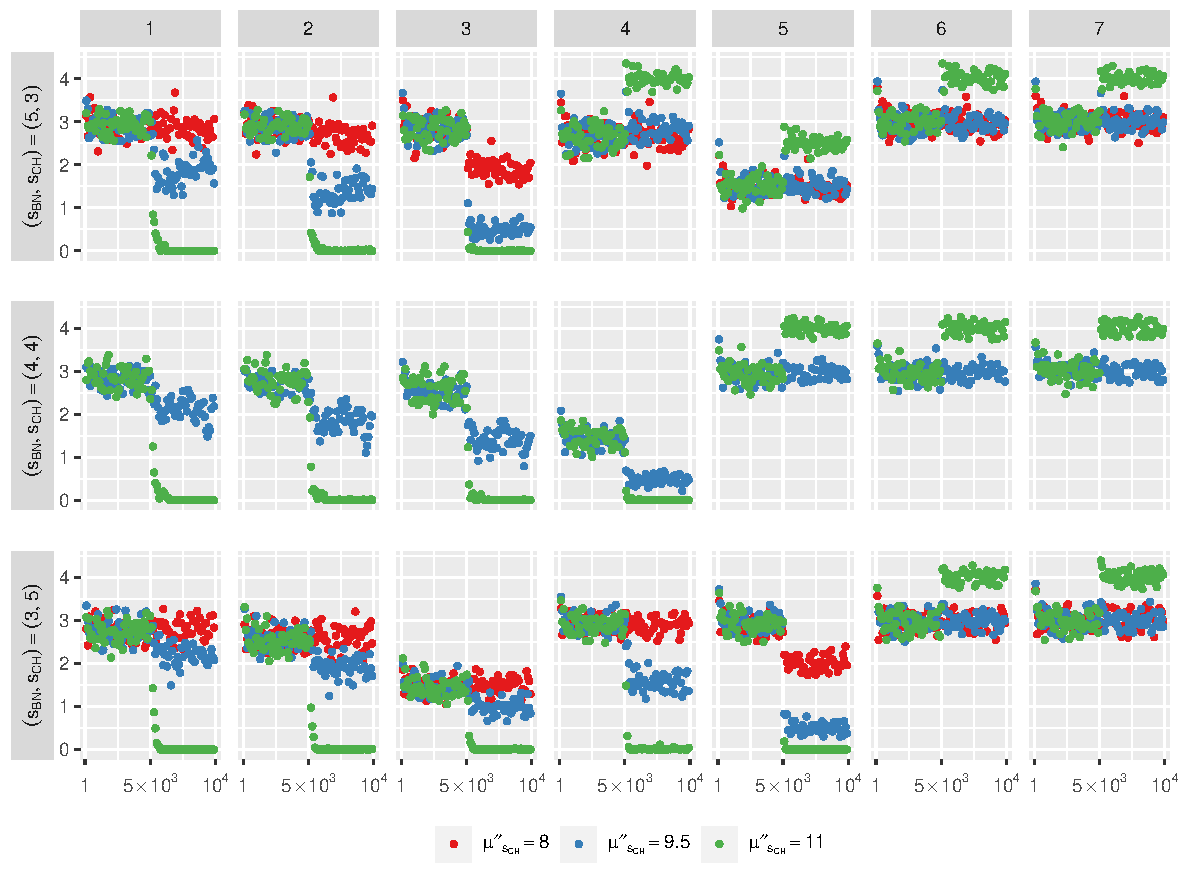
\includegraphics[width=1\textwidth]{ProcessingIncrease8_Starving_time_MEAN}
\caption[Starving time RW KPI behavior with different processing time increase levels]{Starving time RW KPI considering three processing time increase levels $\mu_{s_{CH}}''$ and three bottleneck - changing stage configurations $(s_{BN},s_{CH})$. Models with $cl_s=6$.}
\label{fig:Starving time RW KPI behavior with different processing time increase levels}
\end{figure}
Figures \ref{fig:Blocking time RW KPI behavior with different processing time increase levels} and \ref{fig:Starving time RW KPI behavior with different processing time increase levels} show, respectively, Blocking\_time\_MEAN and Starving\_time\_MEAN RW KPI behaviors when the production capacity of a stage reduces. Looking at these plots it can be said that
\begin{itemize}
\item If a resource loses production capacity to the point that the system becomes unstable:
\begin{itemize}
\item In stages upstream the changing stage $s_{CH}$, average Blocking\_time increases and settles around value $I_s$, while average Starving\_time decreases and settles around value $0$.
\item In correspondence of the changing stage $s_{CH}$, both average Blocking\_time and average Starving\_time decrease and settle around value $0$.
\item In stages downstream the changing stage $s_{CH}$, average Blocking\_time decreases and settles around value $0$, while average Starving\_time increases and settles around value $I_s$.
\end{itemize}
This is visible in models with any configuration $(s_{BN},s_{CH})$ having after-change mean processing time value $\mu_{s_{CH}}''=11$.\\
$I_s$ is equal to the difference between average Mid\_diff and average Processing\_time of stage $s$. In other words, it is a limit that depends on the cycle time as seen in stage $s$, and on stage $s$ production capacity. 
\item If a resource loses production capacity but the system remains stable:
\begin{itemize}
\item In stages upstream the changing stage $s_{CH}$, average Blocking\_time increases towards $I_s$, while average Starving\_time decreases towards $0$.
\item In correspondence of the changing stage $s_{CH}$, both average Blocking\_time and average Starving\_time decrease towards $0$.
\item In stages downstream the changing stage $s_{CH}$, average Blocking\_time decreases towards $0$, while average Starving\_time increases towards $I_s$.
\end{itemize}
This is visible in models with any configuration $(s_{BN},s_{CH})$ having after-change mean processing time value $\mu_{s_{CH}}''=8$ or $\mu_{s_{CH}}''=9.5$.
\item Average Blocking\_time and average Starving\_time variations in a certain stage $s$ are less and less relevant the further stage $s$ is from the changing stage $s_{CH}$, both upstream and downstream $s_{CH}$. 
\item Average Blocking\_time and average Starving\_Queue variations are wider the more significant is the increase of processing time.
\item Average Blocking\_time of stage $s$ stabilizes around the average time a job has to wait in stage $s$ resource after having been processed. \\Average Starving\_time of stage $s$ stabilizes around the average time passing between the exit of a job from stage $s$ resource and the entrance of a new one. \\This is visible in all models, before and after the variation occurring when Case ID reaches value $5000$.
\end{itemize}
Blocking\_time KPI and Starving\_time KPI follow the theoretical behavior of, respectively, blocking and starvation duration. Indeed, in a stable system, blocking is high in stages upstream the bottleneck, and much lower in stages downstream and in correspondence. Conversely, starvation is lower in stages upstream and in correspondence with the bottleneck, and higher downstream. When the system becomes unstable, blocking and starvation behaviors are led to the extreme 
\begin{itemize}
\item Upstream the bottleneck, when buffers become saturated, blocking causes a delay in resource releases, that last until the bottleneck has finished to process a job; so, blocking duration of a certain resource is equal to the time difference between the processing finish of a job in the bottleneck and the processing finish of a job in the considered stage. \\Downstream the bottleneck, since buffers tend to be completely empty, blocking duration drops to $0$.
\item Downstream and in correspondence of the bottleneck, starvation causes resources idleness until the bottleneck has finished to process a job; starvation lasts, like blocking upstream, the time difference between the processing end in the bottleneck and the processing end in the considered stage. \\Upstream the bottleneck, since buffers tend to be completely full, starvation duration drops to $0$.
\end{itemize}
All the observations that have been done regarding these KPIs considering production capacity reductions are similarly valid also in case of production capacity growths.
\begin{figure}[h] 
\centering
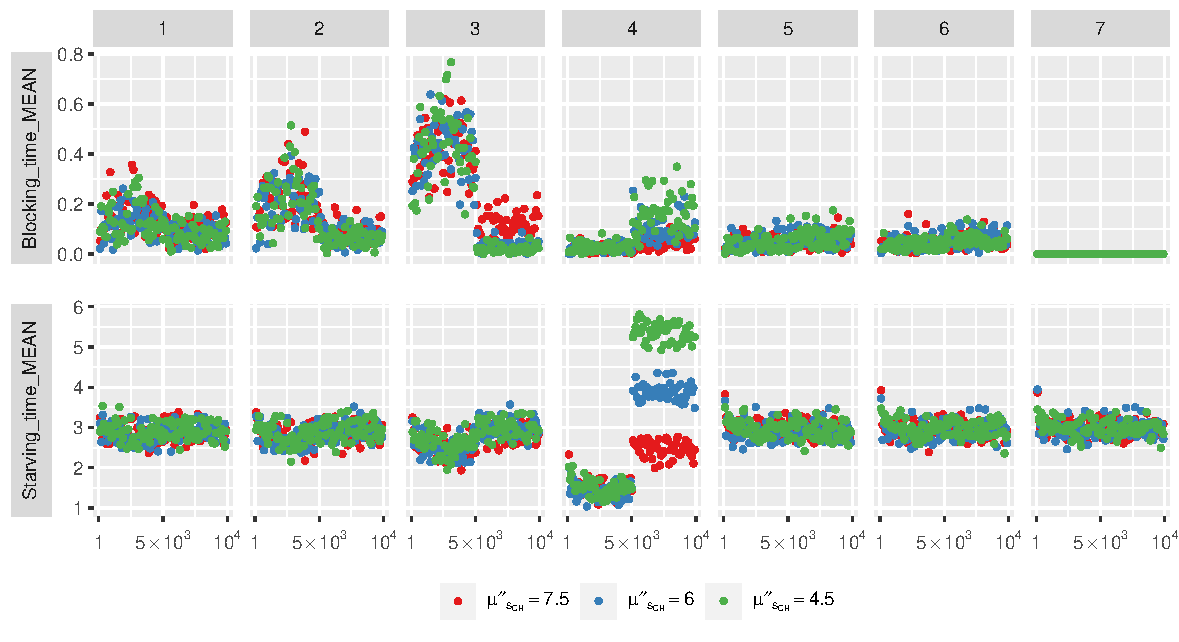
\includegraphics[width=1\textwidth]{ProcessingIncrease11_Blocking_time_MEAN_Starving_time_MEAN}
\caption[Blocking time and Starving time KPI behaviors with different processing time decrease levels]{Blocking time and Starving time KPI behaviors considering three different mean processing time decrease levels $\mu_{s_{CH}}''$. Models with configuration $(s_{BN},s_{CH})=(4,4)$ and $cl_s=6$.}
\label{fig:Blocking time and Starving time KPIs behavior with different processing time decrease levels}
\end{figure}
Figure \ref{fig:Blocking time and Starving time KPIs behavior with different processing time decrease levels} displays average Blocking\_time and average Starving\_time in case a resource processing time decreases. The only difference with the processing time increase case is that average Blocking\_time and average Starving\_time behaviors are inverted when the variation occurs:
\begin{itemize}
\item In stages upstream the changing stage $s_{CH}$, average Blocking\_time decreases, while average Starving\_time increases.
\item In correspondence of the changing stage $s_{CH}$, both average Blocking\_time and average Starving\_time increase.
\item In stages downstream the changing stage $s_{CH}$, average Blocking\_time increases, while average Starving\_time decreases.
\end{itemize}
\subsubsection{Blocking\_time and Starving\_time KPIs considering different buffer levels}
Previously only one buffer capacity limit ($cl_s=6$) was taken into account in the analysis. However, Blocking\_time and Starving\_time KPIs are also influenced by the buffer capacity, and it is interesting to study their behavior considering different capacity levels.
\begin{figure}[h] 
\centering
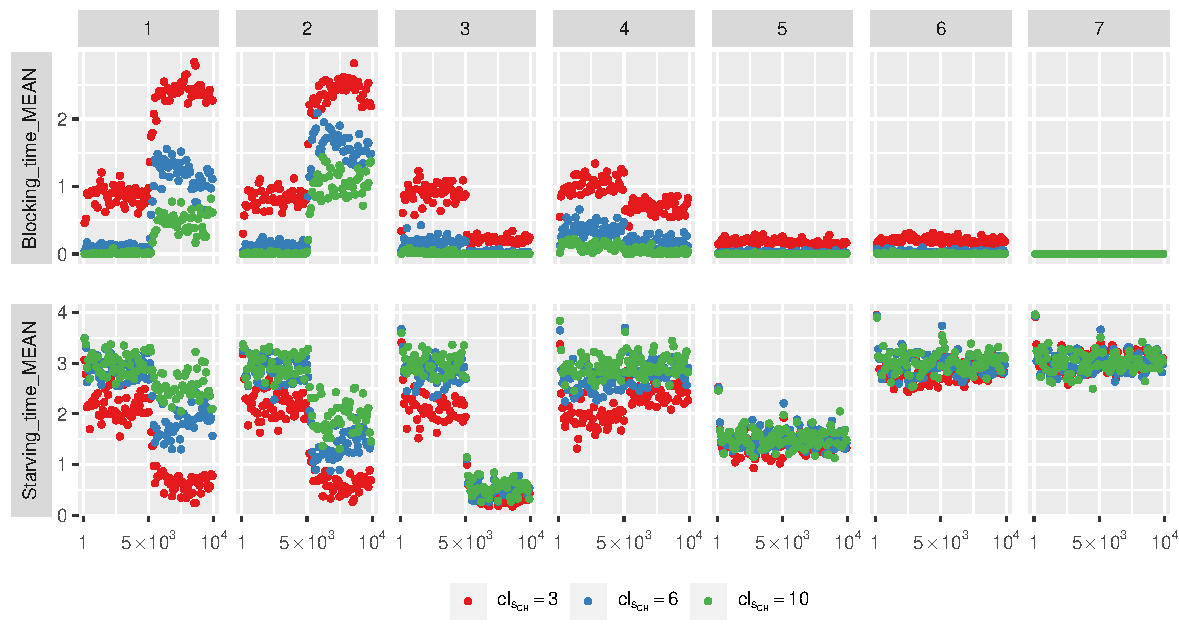
\includegraphics[width=1\textwidth]{ProcessingIncrease9_Blocking_time_MEAN_Starving_time_MEAN}
\caption[Blocking time and Starving time RW KPIs behaviors in case of processing time increase considering different buffer capacity limits]{Blocking time and Starving time RW KPI behaviors in case of mean processing time increase $\mu_{s_{CH}}''$ considering different buffer capacity limits $cl_s$. Models with configuration $(s_{BN},s_{CH})=(5,3)$ and $\mu_{s_{CH}}''=9.5$.}
\label{fig:Blocking time and Starving time RW KPIs behavior in case of processing time increase considering different buffer capacity limits}
\end{figure}
Figure \ref{fig:Blocking time and Starving time RW KPIs behavior in case of processing time increase considering different buffer capacity limits} shows average Blocking\_time and average Starving\_time behaviors in case of a processing time increase, but considering models having three different buffer capacity limits $cl_s$. \\
When a stage loses production capacity:
\begin{itemize}
\item The variation extents of average Blocking\_time and average Starving\_time are wider the lower the buffer capacity limit is
\item The variation extents of average Blocking\_time and average Starving\_time are narrower the higher the buffer capacity limit is
\end{itemize}
It is particularly visible comparing the model with $cl_s=3$ and the one with $cl_s=6$. \\
This happens because smaller buffers are on average easily saturated, causing longer resource blockings in previous stages and reducing starvation. When buffers are bigger the opposite verifies.
\subsubsection{Value $I_s$ behavior and Blocking\_time and Starving\_time relative proportions}
It is noteworthy to explain that value $I_s$ \footnote{Remember that $I_s$ was defined as the difference between average Mid\_diff and average Processing\_time of stage $s$} is not simply a superior limit for average Blocking\_time or average Starving\_time, but actually it is always equal to their sum. As a matter of fact, the sum of Blocking\_time and Starving\_time of stage $s$ is always equal to the difference between Mid\_diff and Processing\_time of stage $s$ because of how these KPIs are defined (see subsection \ref{Derived KPIs}). 
\[Blocking\_time(j,s)+Starving\_time(j,s)=Mid\_diff(j,s)-Processing\_time(j,s)\]
Theoretically, this is reasonable given the characteristics of the considered systems: since machine breakdowns are assumed to never occur, resources can find themselves in three possible states, which are seized and working state (processing), seized and not working state (blocking), and not seized state (starvation). Sum of the total time spent by a resource in these states gives the whole available time of the resource, as, analogously, Processing\_time, Blocking\_time, and Starving\_time add up matching Mid\_diff. 
\begin{figure}[h] 
\centering
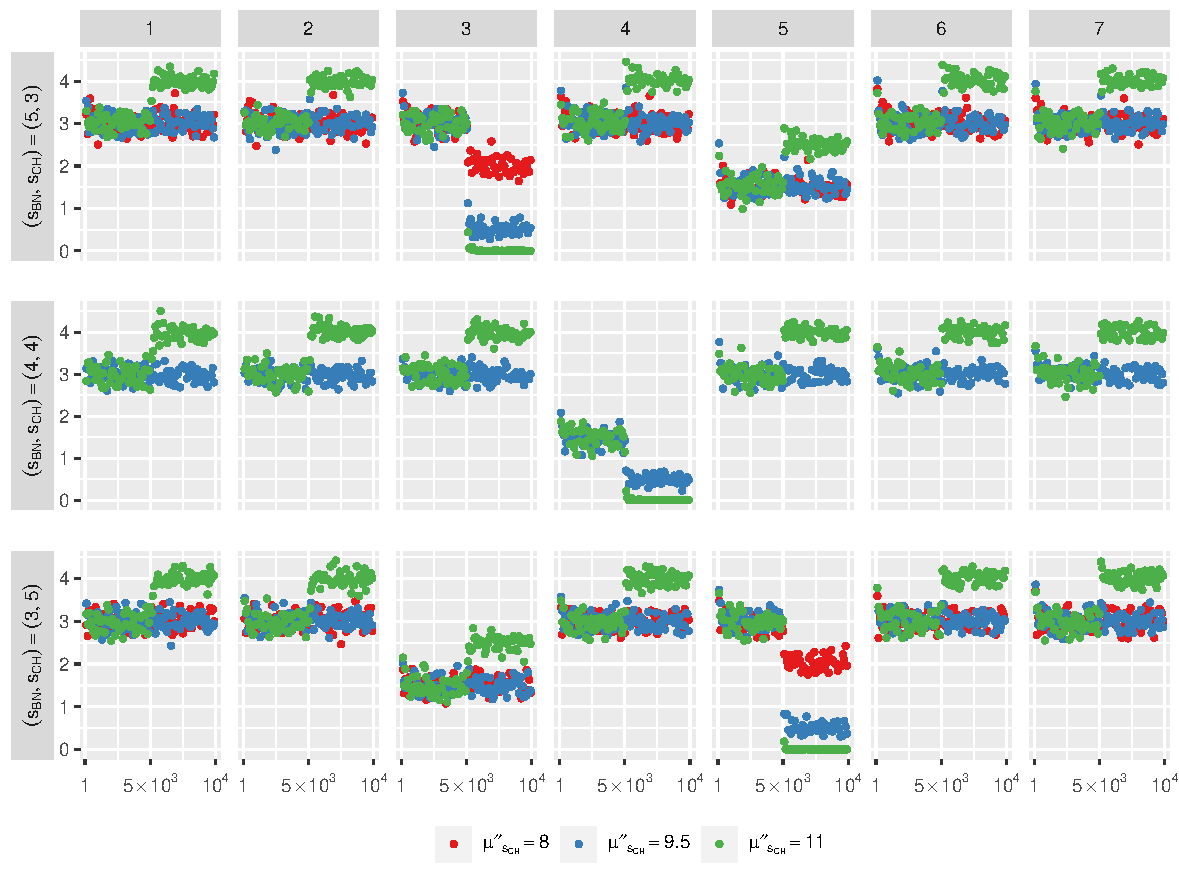
\includegraphics[width=1\textwidth]{ProcessingIncrease17_Blocking_time_MEAN_Starving_time_MEAN}
\caption[Value $I_s$ behavior with different processing time increase levels]{Value $I_s$ considering three different mean processing time increase levels $\mu_{s_{CH}}''$ and three bottleneck - changing stage configurations $(s_{BN},s_{CH})$. Models with $cl_s=6$.}
\label{fig:Value $I_s$ behavior with different processing time increase levels}
\end{figure}
Figure \ref{fig:Value $I_s$ behavior with different processing time increase levels} is helpful to understand how $I_s$ behaves.
\begin{itemize}
\item If a production capacity variation occurs, but the system remains stable, average $I_s$ changes only in correspondence of the changing stage $s_{CH}$ (it reduces if $\mu_{s_{CH}}''>\mu_{s_{CH}}'$, increases if $\mu_{s_{CH}}''<\mu_{s_{CH}}'$). \\It is visible in models with $\mu_{s_{CH}}''=8$ or $\mu_{s_{CH}}''=9.5$.
\item If a production capacity variation occurs and the system becomes unstable, average $I_s$ drops to $0$ in correspondence with the changing stage $s_{CH}$, and grows in all other stages. \\It is visible in models with $\mu_{s_{CH}}''=11$.
\end{itemize}
Since $I_s$ is also the sum of average Blocking\_time and average Starving\_time, this means that the sum of these KPIs, if the system remains stable, is constant in all stages except for the changing stage $s_{CH}$. Instead, if the system becomes unstable, the sum reduces to $0$ in $s_{CH}$ and grows in all other stages. At this point, it is interesting to visualize the relative proportions of Blocking\_time and Starving\_time in this sum. 
\begin{figure}[h] 
\centering
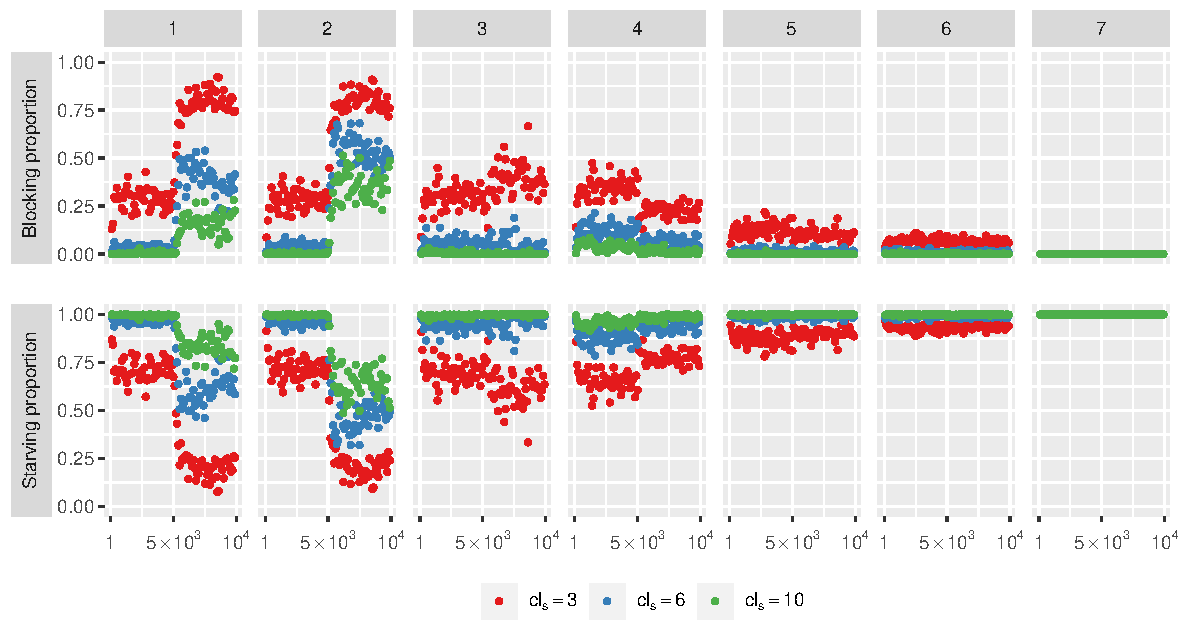
\includegraphics[width=1\textwidth]{ProcessingIncrease18_Blocking_prop_Starving_prop}
\caption[Average Blocking time and Starving time relative proportions considering different buffer capacity limits]{Average Blocking time and Starving time relative proportions considering different buffer capacity limits $cl_s$. Models with configurations $(s_{BN},s_{CH})=(5,3)$, and after-change mean processing time $\mu_{s_{CH}}''=9.5$.}
\label{fig:Average Blocking time and Starving time relative proportions considering different buffer capacity limits}
\end{figure}
Figure \ref{fig:Average Blocking time and Starving time relative proportions considering different buffer capacity limits} shows that 
\begin{itemize}
\item The contribution of average Blocking\_time in $I_s$ increases the smaller is the buffer.
\item The contribution of average Starving\_time in $I_s$ reduces the smaller is the buffer.
\end{itemize}
\subsubsection{Blocking\_prob and Starving\_prob KPIs}
Like Processing\_time, also Blocking\_time and Starving\_time can be represented in combination with Mid\_diff. The obtained KPIs are Blocking\_prob and Starving\_prob.
\begin{figure}[h] 
\centering
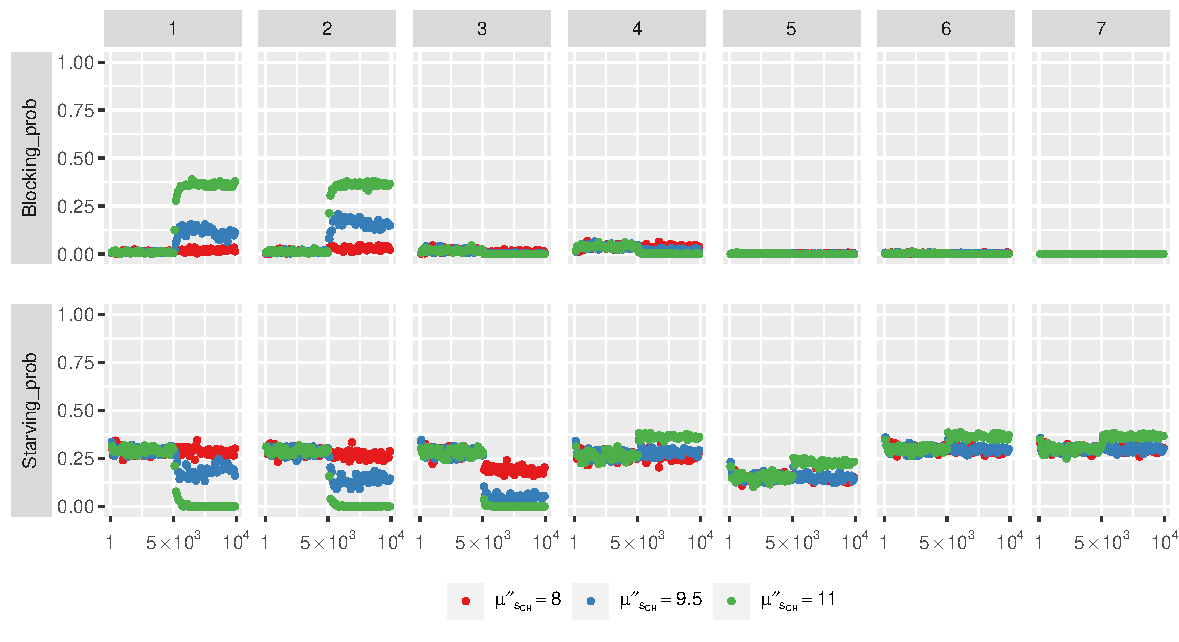
\includegraphics[width=1\textwidth]{ProcessingIncrease10_Blocking_prob_Starving_prob}
\caption[Blocking prob and Starving prob KPI behaviors with different processing time increase levels]{Blocking prob and Starving prob KPI behaviors considering three processing time increase levels $\mu_{s_{CH}}''$. Models with configurations $(s_{BN},s_{CH})=(5,3)$ and $cl_s=6$.}
\label{fig:Blocking prob and Starving prob KPIs behavior with different processing time increase levels}
\end{figure}
Figure \ref{fig:Blocking prob and Starving prob KPIs behavior with different processing time increase levels} portrays an example of these KPIs. These KPIs indicate how much of the available time was spent by the resources without being utilized. The observations that can be made regarding these KPI behaviors are analogous to one done for Blocking\_time and Starving\_time. 
\newpage
\subsection{Waiting\_time and Average\_Queue KPIs}
\label{Waiting time and Average Queue KPIs - Processing time variation}
Blocking\_time and Starving\_time help to monitor the effects of a variation on the exploitation of resources in stages different from the changing stage; indirectly, these KPIs allow to get insights about the buffer saturation levels. However, to get a closer and more precise view of job queues statuses, it is necessary to resort to Waiting\_time KPI. In this subsection, firstly Waiting\_time and Average\_Queue, which is its derived Stage State KPI, behaviors are discussed; then, at the end, the effects of having an unlimited buffer in the first stage are briefly addressed.
\subsubsection{Processing time increase effects on Waiting\_time KPI}
\begin{figure}[h] 
\centering
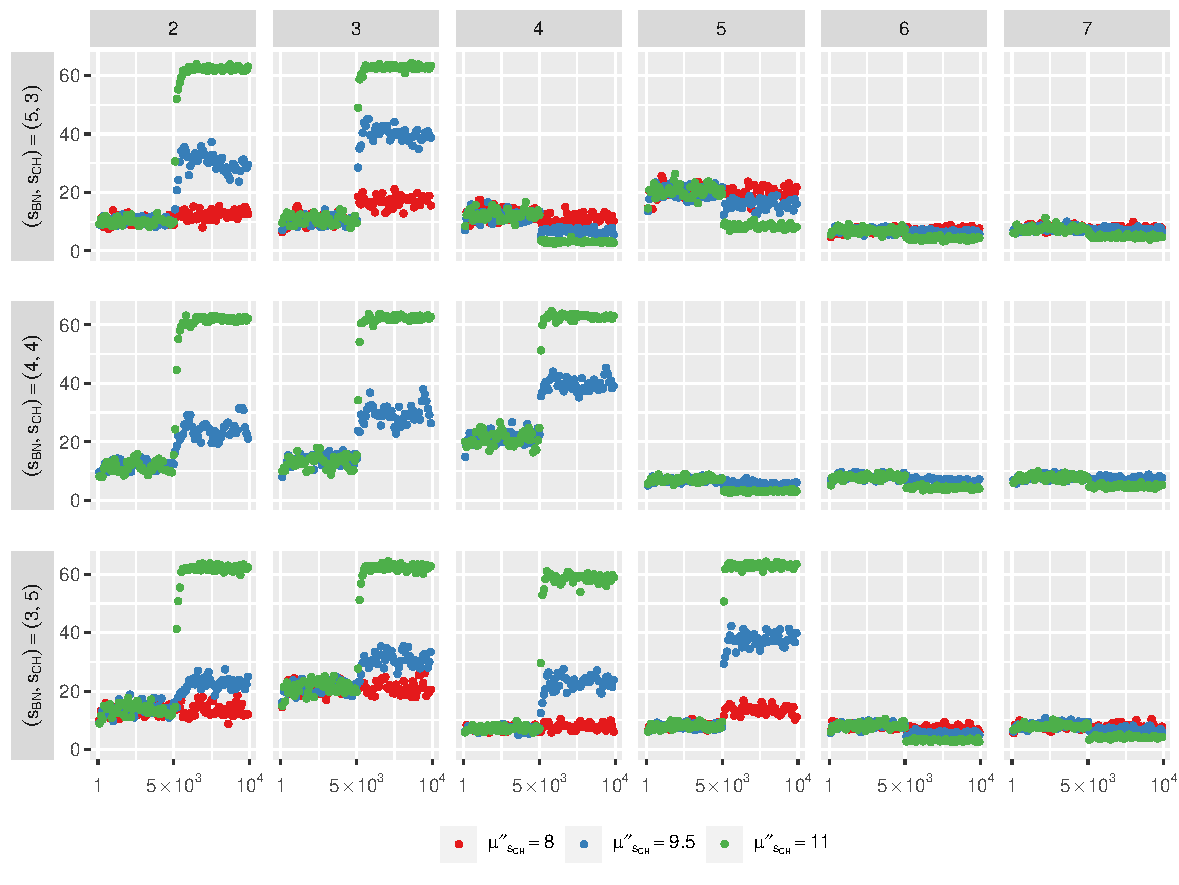
\includegraphics[width=1\textwidth]{ProcessingIncrease12_Waiting_time_MEAN}
\caption[Waiting time RW KPI behavior with different processing time increase levels]{Waiting time RW KPI behavior considering three processing time increase levels $\mu_{s_{CH}}''$ and three bottleneck - changing stage configurations $(s_{BN},s_{CH})$. Models with $cl_s=6$.}
\label{fig:Waiting time KPI behavior with different processing time increase levels}
\end{figure}
Figure \ref{fig:Waiting time KPI behavior with different processing time increase levels} the behavior of Waiting\_time\_MEAN RW KPI in case of a production capacity decrease in a stage. 
\begin{itemize}
\item If a resource loses production capacity to the point that the system becomes unstable:
\begin{itemize}
\item In stages upstream the changing stage $s_{CH}$, average Waiting\_time increases and settles around value $LW_s$.
\item In correspondence of the changing stage $s_{CH}$, average Waiting\_time increases and settles around value $LW_s$.
\item In stages downstream the changing stage $s_{CH}$, average Waiting\_time decreases towards $0$.
\end{itemize}
This is visible in models with any configuration $(s_{BN},s_{CH})$ having after-change mean processing time value $\mu_{s_{CH}}''=11$.\\
$LW_s$ is equal to the product of average Input\_diff and the maximum buffer capacity of stage $s$, $cl_s$. In other words, it is a limit that depends on the cycle time as seen in stage $s$, and on stage $s$ buffer capacity. 
\item If a resource loses production capacity but the system remains stable:
\begin{itemize}
\item In stages upstream the changing stage $s_{CH}$, average Waiting\_time increases.
\item In correspondence of the changing stage $s_{CH}$, average Waiting\_time increases.
\item In stages downstream the changing stage $s_{CH}$, average Waiting\_time decreases.
\end{itemize}
This is visible in models with any configuration $(s_{BN},s_{CH})$ having after-change mean processing time value $\mu_{s_{CH}}''=8$ or $\mu_{s_{CH}}''=9.5$.
\item Average Waiting\_time variations are wider the more significant is the increase of processing time.
\item Average Waiting\_time variations in a certain stage $s$ are less and less relevant the further stage $s$ is from the changing stage $s_{CH}$, both upstream and downstream $s_{CH}$. 
\item Average Waiting\_time of stage $s$ stabilizes around the average time a job has to wait in stage $s$ buffer before seizing the resource. \\This is visible in all models, before and after the variation occurring when Case ID reaches value $5000$.
\end{itemize}
Average Waiting\_time of stage $s$ follows the theoretical behavior of the average time a job spends in stage $s$ buffer. Indeed, the time a job has to wait is longer in stages upstream and in correspondence with the bottleneck and lower in stages downstream. Moreover, if the system becomes unstable, buffers in stages upstream and in correspondence with the bottleneck get saturated, and the job queue is longer the higher the buffer capacity limit is. Since jobs in buffers, before seizing the resource, have to wait until all other jobs which have entered before them are processed\footnote{The service policy was assumed to be FIFO, see section \ref{Considered systems}}, the time they have to wait is equal to the number of jobs in the queue before them (which is equal to the buffer limit, since it is full) multiplied by the job inter-arrival time in the queue, that is the cycle time.
\subsubsection{Value $LW_s$ and Average\_Queue KPI}
$LW_s$ has been defined as a limit value for stage $s$ average Waiting\_time if the system becomes unstable, however its equation can be generalized to be also valid when the system works in a stable condition. Indeed, theory says that the job average waiting time in a queue is always equal to the average cycle time multiplied by the average number of jobs in the queue. This means that average Waiting\_time of stage $s$ is always equal to the product of stage $s$ average Input\_diff\footnote{Input\_diff is the indicator of the cycle time as it is seen at buffer entrances} and the average number of jobs in stage $s$ buffer. $LW_s$ is just the value taken by average Waiting\_time in stages upstream the bottleneck when a particular situation occurs, that is when system becomes unstable. \\
This observation explains why Average\_queue (i.e. the ratio between average Waiting\_time and Input\_diff, see subsection \ref{Derived KPIs}) indicates the average number of jobs in a buffer.
\begin{figure}[h] 
\centering
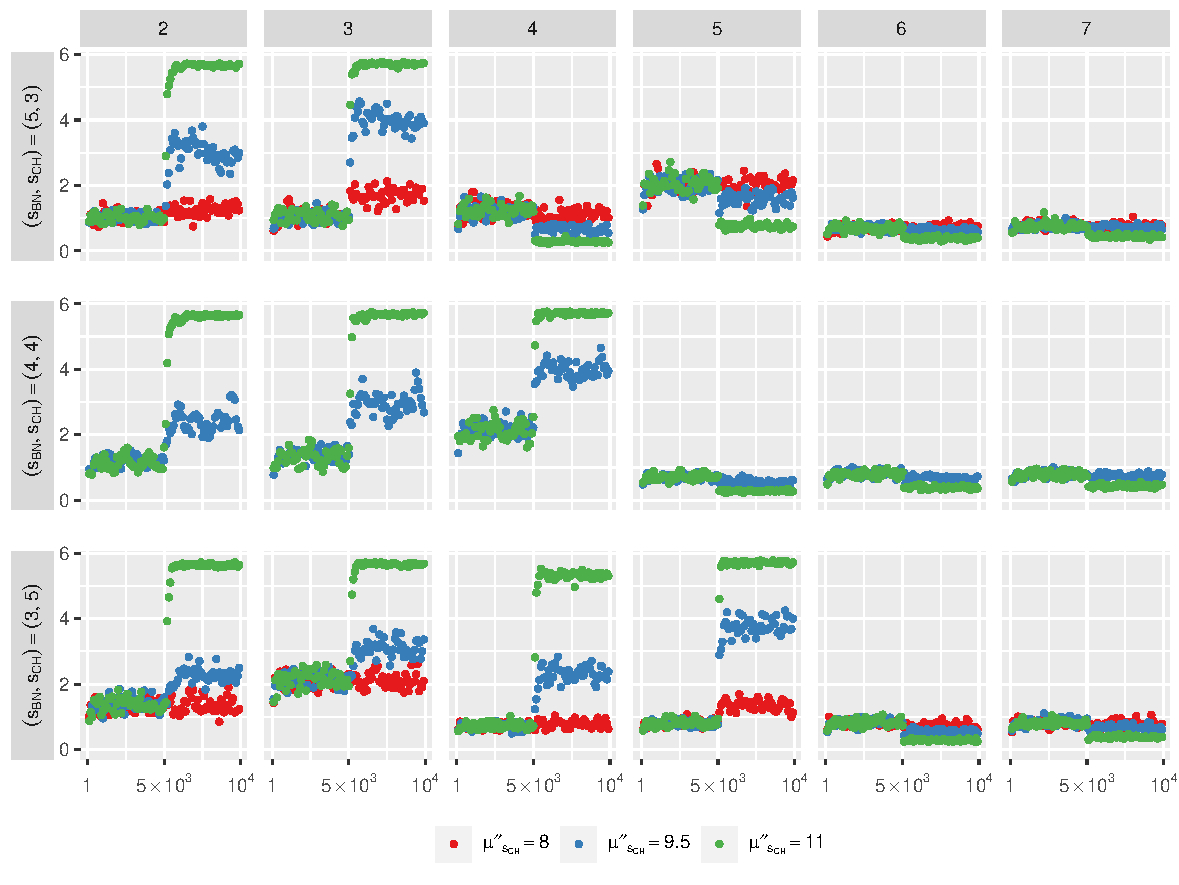
\includegraphics[width=1\textwidth]{ProcessingIncrease13_Average_Queue}
\caption[Average Queue KPI behavior with different processing time increase levels]{Average Queue KPI behavior considering three processing time increase levels $\mu_{s_{CH}}''$ and three bottleneck - changing stage configurations $(s_{BN},s_{CH})$. Models with $cl_s=6$.}
\label{fig:Average Queue KPI behavior with different processing time increase levels}
\end{figure}
Figure \ref{fig:Average Queue KPI behavior with different processing time increase levels} portrays Average\_Queue considering the same models of figure \ref{fig:Waiting time KPI behavior with different processing time increase levels}. This KPI behavior is similar to the Waiting\_time one 
\begin{itemize}
\item If a resource loses production capacity to the point that the system becomes unstable:
\begin{itemize}
\item In stages upstream the changing stage $s_{CH}$, Average\_Queue increases and settles around the buffer capacity limit $cl_s$.
\item In correspondence of the changing stage $s_{CH}$, Average\_Queue increases and settles around the buffer capacity limit $cl_{s_{CH}}$.
\item In stages downstream the changing stage $s_{CH}$, Average\_Queue decreases towards $0$.
\end{itemize}
This is visible in models with any configuration $(s_{BN},s_{CH})$ having after-change mean processing time value $\mu_{s_{CH}}''=11$.
\item If a resource loses production capacity but the system remains stable:
\begin{itemize}
\item In stages upstream the changing stage $s_{CH}$, Average\_Queue increases towards the buffer capacity limit $cl_s$.
\item In correspondence of the changing stage $s_{CH}$, Average\_Queue increases towards the buffer capacity limit $cl_{s_{CH}}$.
\item In stages downstream the changing stage $s_{CH}$, Average\_Queue decreases towards $0$.
\end{itemize}
This is visible in models with any configuration $(s_{BN},s_{CH})$ having after-change mean processing time value $\mu_{s_{CH}}''=8$ or $\mu_{s_{CH}}''=9.5$.
\item Average\_Queue variations are wider the more significant is the decrease of processing time.
\item Average\_Queue variations in a certain stage $s$ are less and less relevant the further stage $s$ is from the changing stage $s_{CH}$, both upstream and downstream. 
\item Average\_Queue of stage $s$ stabilizes around the average number of jobs present in stage $s$ buffer. \\This is visible in all models, before and after the variation occurring when Case ID reaches value $5000$.
\end{itemize}
\subsubsection{Waiting\_time behavior considering different buffer sizes}
As said before, Waiting\_time and Average\_Queue behaviors depend on buffer capacity limits. However, the buffer limitation does not affect these KPIs only when the system is unstable (i.e. when Waiting\_time reaches its limit $LW_s$ and Average\_Queue settles around the buffer maximum capacity $cl_s$), but it can influence them also when the system is stable. For sake of brevity, since Waiting\_time and Average\_Queue behaviors are very similar, only plots of the first one are displayed.
\begin{figure}[h] 
\centering
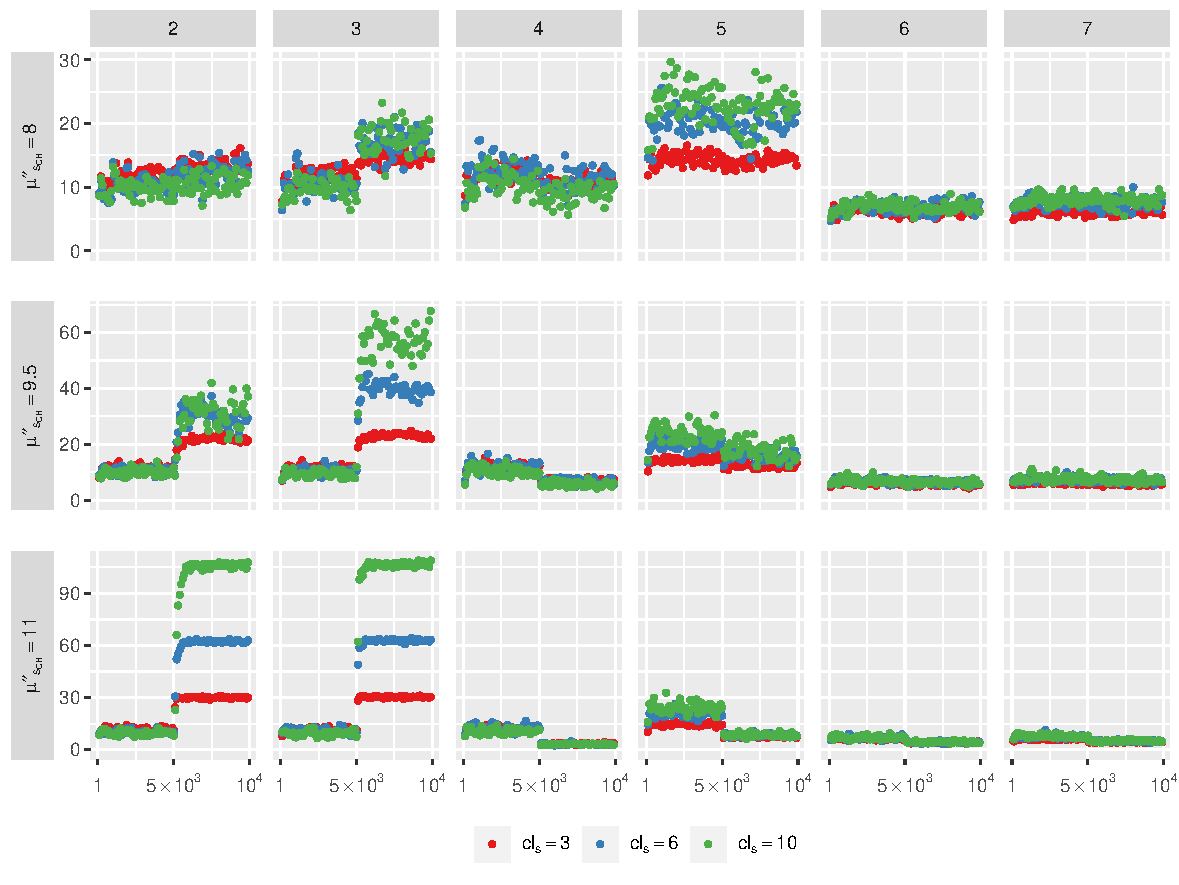
\includegraphics[width=1\textwidth]{ProcessingIncrease14_Waiting_time_MEAN}
\caption[Average Waiting time KPI behavior with different processing time increase levels considering different buffer capacity limits]{Average Waiting time KPI behavior considering three different mean processing time increase levels $\mu_{s_{CH}}$ and three buffer capacity limits $cl_s$. Models with configuration $(s_{BN},s_{CH})=(5,3)$.}
\label{fig:Average Waiting time KPI behavior with different processing time increase levels considering different buffer capacity limits}
\end{figure}
Figure \ref{fig:Average Waiting time KPI behavior with different processing time increase levels considering different buffer capacity limits} shows Waiting\_time in case of production capacity loss, considering three different buffer limits $cl_s$. Since the influence of buffer capacity limits on Waiting\_time and Average\_Queue behaviors is quite complex and an in-depth analysis falls outside the goal of this thesis, the observations here listed are always valid but insufficient to fully describe this dependence.
\begin{itemize}
\item When a resource loses production capacity, the higher the capacity limit $cl_s$ is, the wider the increase of average Waiting\_time in correspondence of the changing stage $s_{CH}$. \\This is visible in correspondence with the changing stage $s_{CH}=3$, comparing models with different buffer capacity limits $cl_s$.
\item When a resource loses production capacity but the system remains stable, the higher the capacity limit $cl_s$ is, the less relevant the spread of average Waiting\_time variation is in stages upstream and downstream the changing stage $cl_s$. \\This is visible upstream and downstream the changing stage $s_{CH}=3$, comparing models with different buffer capacity limits $cl_s$, having after-change mean processing time value $\mu_{s_{CH}}''=8$ or $\mu_{s_{CH}}''=9.5$.
\end{itemize}
To observe another impact of buffer capacity limits on Waiting\_time, systems with unlimited buffer are briefly considered. Indeed, even if it is not a realistic condition, it can be interpreted as a case of systems having buffers with extremely high capacity limits. 
\begin{figure}[h] 
\centering
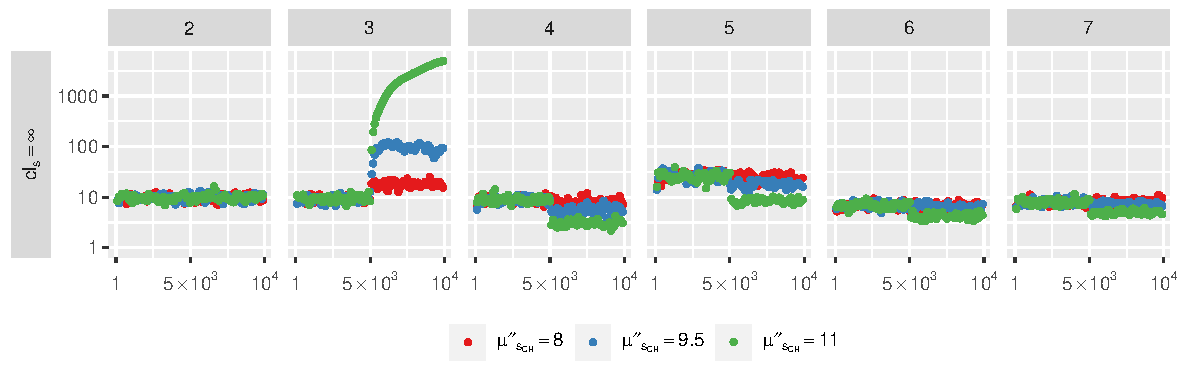
\includegraphics[width=1\textwidth]{ProcessingIncrease19_Waiting_time_MEAN}
\caption[Average Waiting time KPI behavior with different processing time increase levels considering buffers with unlimited capacity]{Average Waiting time KPI behavior considering three different mean processing time increase levels $\mu_{s_{CH}}$ and buffers with unlimited capacity. Models with configuration $(s_{BN},s_{CH})=(5,3)$ and $cl_s=\infty$. Graphs with log-scale on y-axis.}
\label{fig:Average Waiting time KPI behavior with different processing time increase levels considering buffers with unlimited capacity}
\end{figure}
Figure \ref{fig:Average Waiting time KPI behavior with different processing time increase levels considering buffers with unlimited capacity} shows average Waiting\_time behavior in case of a production capacity decrease when all buffers have unlimited capacity. The effects of high capacity buffers are taken to the extreme: when the changing stage $s_{CH}$ processing time increases, average Waiting\_time extensively decreases in stages downstream $s_{CH}$ and increases in correspondence with the changing stage $s_{CH}$. If, after the variation, the system becomes unstable (as in model with $\mu_{s_{CH}}''=11$), average Waiting\_time of stage $s_{CH}$ even grows towards infinity, since buffers have no boundaries and job mean inter-arrival in the first stage is lower than the mean processing time of the changing stage ($\mu_a<\mu_{s_{CH}}''$). However, it can be noticed that Waiting\_time does not change in stage $s=2$, upstream $s_{CH}$, even when the system becomes unstable. 
\\ The discussion about this particular (not realistic) case was included to show that buffers having high capacity limits work as temporary decoupling points, delaying variation effects on KPIs to spread upstream the stage in which they are positioned. The delay caused by infinite buffers (which are permanent decoupling points) is infinite, and so KPIs upstream never change.
\subsubsection{Processing time decrease effects on Waiting\_time and Average\_Queue KPIs}
The effects of a production capacity increase on Waiting\_time and Average\_Queue KPIs are the opposite than the ones caused by a production capacity decrease.
\begin{figure}[h] 
\centering
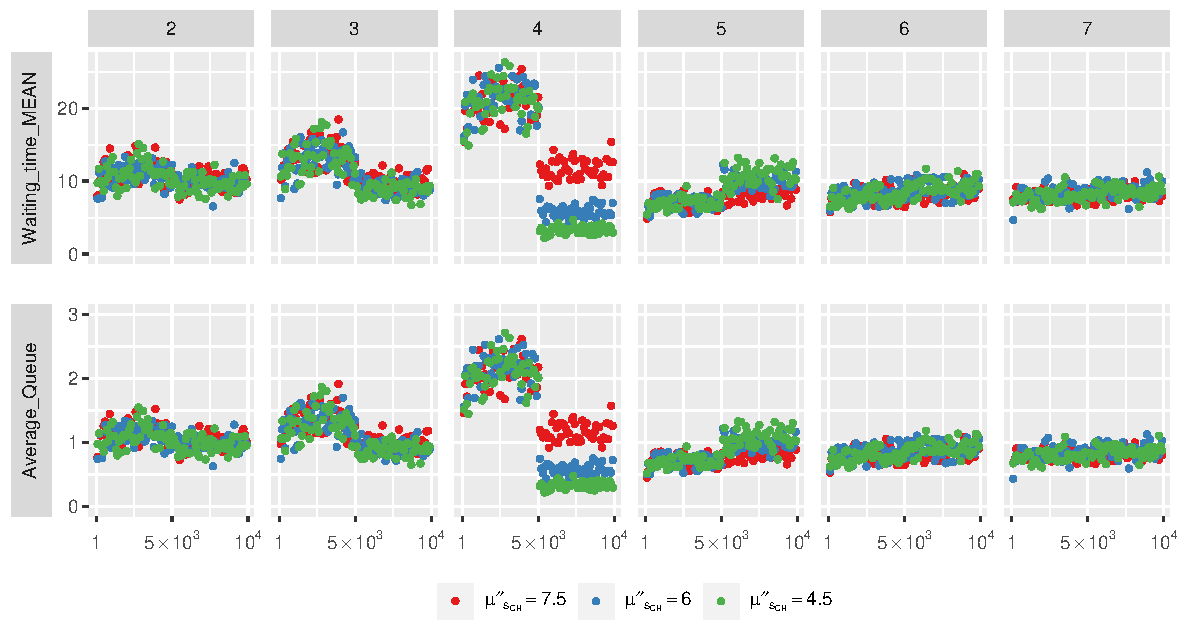
\includegraphics[width=1\textwidth]{ProcessingIncrease15_Waiting_time_MEAN_Average_Queue}
\caption[Waiting time RW and Average Queue KPIs behaviors with different processing time decrease levels]{Waiting time RW and Average Queue KPIs behaviors considering different processing time decrease levels $\mu_{s_{CH}}''$. Models with configuration $(s_{BN},s_{CH})=(4,4)$ and $cl_s=6$.}
\label{fig:Waiting time RW and Average Queue KPIs behaviors with different processing time decrease levels}
\end{figure}
Figure \ref{fig:Waiting time RW and Average Queue KPIs behaviors with different processing time decrease levels} shows Waiting\_time and Average\_Queue behaviors in case of a mean processing time $\mu_{s_{CH}}$ decrease. 
\begin{itemize}
\item If a resource increases its production capacity 
\begin{itemize}
\item In stages upstream the changing stage $s_{CH}$, average Waiting\_time and Average\_Queue decrease.
\item In correspondence of the changing stage $s_{CH}$, average Waiting\_time and Average\_Queue decrease.
\item In stages downstream the changing stage $s_{CH}$, average Waiting\_time and Average\_Queue increase.
\end{itemize}
\item Average Waiting\_time and Average\_Queue variations are wider the more significant is the increase of processing time.
\item Average Waiting\_time and Average\_Queue variations in a certain stage $s$ are less and less relevant the further stage $s$ is from the changing stage $s_{CH}$, both upstream and downstream. 
\end{itemize}
\subsubsection{Waiting\_time and Average\_Queue KPI behaviors in the first stage of the line}
It should be noted that the first stage has not been included in any figure of this subsection. As a matter of fact, since the first stage buffer is unlimited, the information of how much time jobs spend in it and how many are present at the same time is not useful. Moreover, Waiting\_time and Average\_Queue of the first stage infinitely grow when the system becomes unstable, a circumstance in which Average\_Queue even becomes a wrong indicator of the average number of jobs in the buffer.
\begin{figure}[h] 
\centering
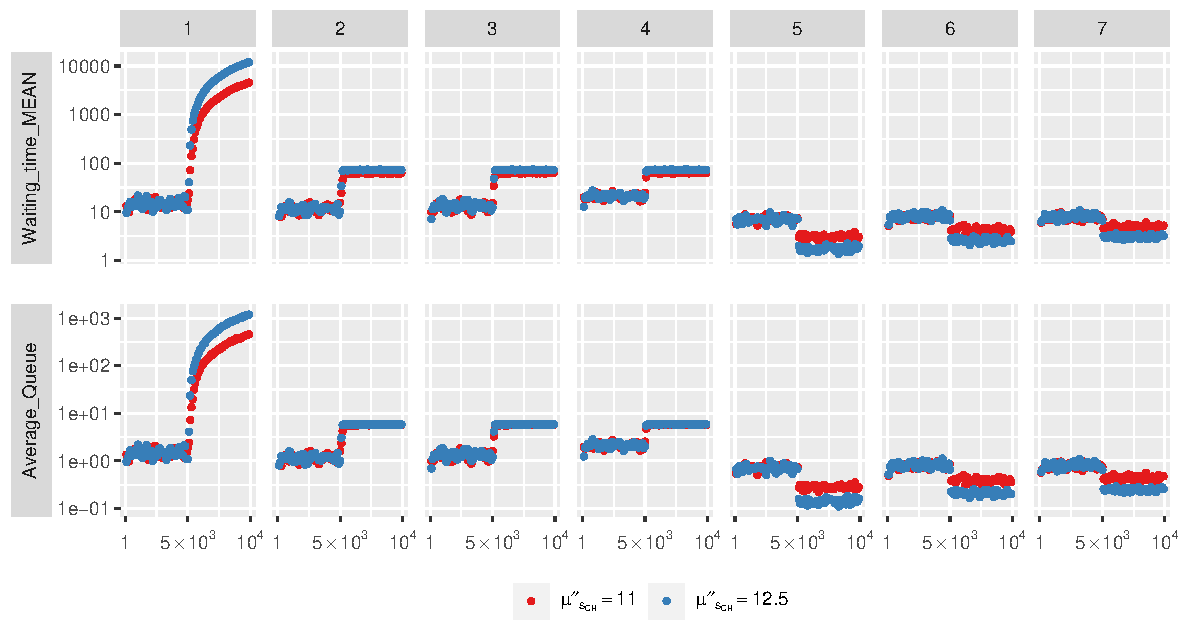
\includegraphics[width=1\textwidth]{ProcessingIncrease16_Waiting_time_MEAN_Average_Queue}
\caption[Waiting time RW and Average Queue KPIs behaviors with different processing time increase levels that make the system unstable]{Waiting time RW and Average Queue KPIs behaviors considering different processing time increase levels that make the system unstable. Models with configuration $(s_{BN},s_{CH})=(4,4)$ and $cl_s=6$. Graphs with log-scale on y-axis.}
\label{fig:Waiting time RW and Average Queue KPIs behaviors with different processing time increase levels that make the system unstable}
\end{figure}
Figure \ref{fig:Waiting time RW and Average Queue KPIs behaviors with different processing time increase levels that make the system unstable} shows the behaviors of Waiting\_time and Average\_Queue when the system becomes unstable: in the first stage both these KPIs increase towards infinity. In particular it should be noticed that, at the end of the process, but Average\_Queue grows as if new jobs kept arriving, even if no more jobs enter the line and the buffer starts emptying. This error verifies because in this situation Waiting\_time (rightly) keeps increasing, yet Input\_diff remains equal to the bottleneck processing time. Reminding how Average\_Queue is computed, this means that the numerator keeps growing while the denominator is fixed, making the KPI erroneously continuously increasing. \\Because of these irregular behaviors, first stage plots have been omitted in previous figures. 
\newpage
\section{Buffer capacity variation}
A buffer capacity variation does not have effects on resource processing time and, so, never influences the system cycle time. Therefore, this type of variation is visible only in KPIs related to buffers (i.e. Waiting\_time, Blocking\_time and Starving\_time, and the relative Stage State KPIs), while the others (CCI KPIs, Processing\_time and Utilization) are not subject to any change. Plots of KPIs not influenced by buffer capacity variations are not shown and discussed, to restrain the analysis to the most relevant indicators.
\subsection{Waiting\_time KPI}
\label{Waiting time KPI - Buffer capacity variation}
Waiting\_time and Average\_Queue are strongly influenced by buffer capacity limits (as shown in subsection \ref{Waiting time and Average Queue KPIs - Processing time variation}) and are directly related to queue statuses. In this subsection Waiting\_time behavior is analyzed in situations where a buffer capacity variation verifies, while Average\_Queue is not discussed, since it shows the same behavior of Waiting\_time. At the end of the subsection the problem of buffers having high capacity limits before the capacity variation is presented.
\subsubsection{Buffer capacity increase effects on Waiting\_time KPI}
\begin{figure}[h] 
\centering
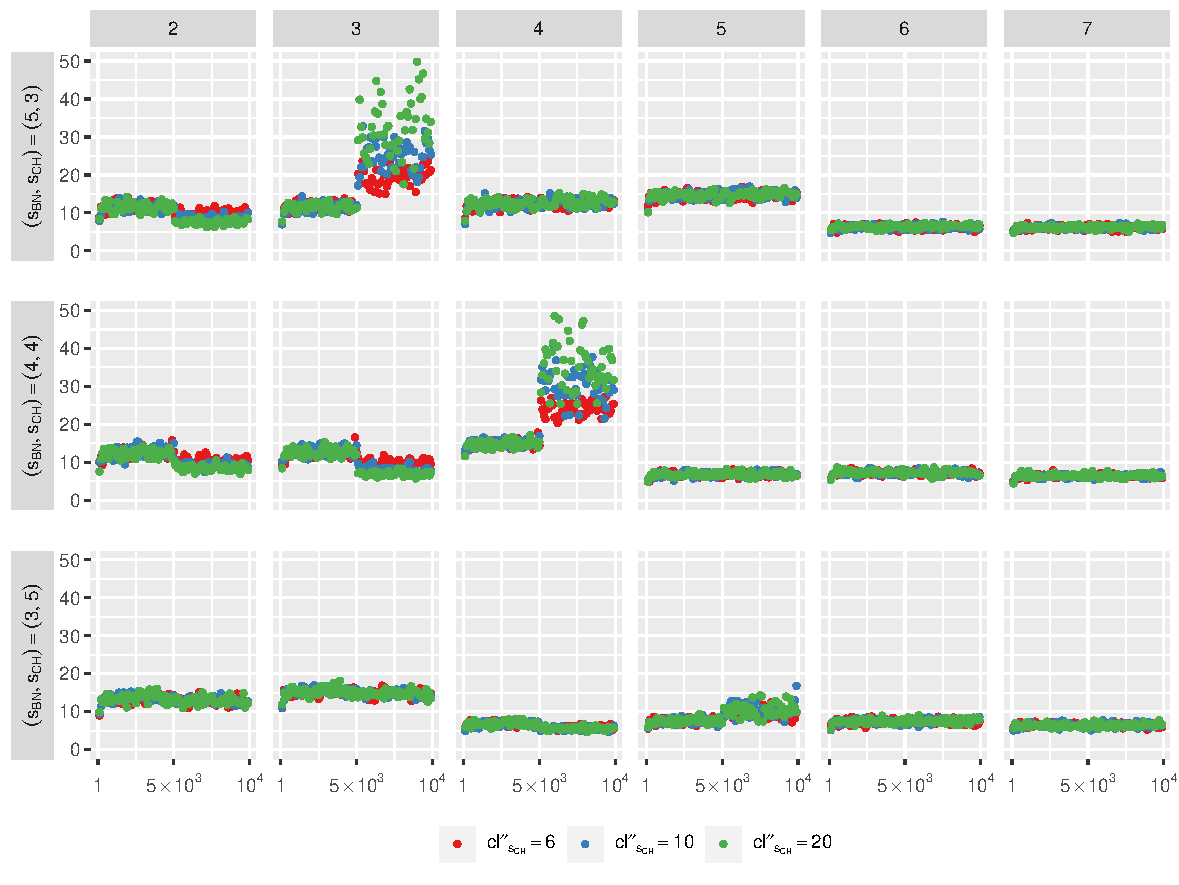
\includegraphics[width=1\textwidth]{BufferIncrease1_Waiting_time_MEAN}
\caption[Waiting time RW KPI behavior with different buffer capacity increase levels]{Waiting time RW KPI behavior considering different buffer capacity increase levels $cl_{s_{CH}}''$ and three bottleneck - changing stage configurations $(s_{BN},s_{CH})$. Models with $cl_s'=3$.}
\label{fig:Waiting time RW KPI behavior with different buffer capacity increase levels}
\end{figure}
Figure \ref{fig:Waiting time RW KPI behavior with different buffer capacity increase levels} shows average Waiting\_time behavior when a buffer capacity increases.
\begin{itemize}
\item If a buffer capacity increases
\begin{itemize}
\item In stages upstream the changing stage $s_{CH}$, average Waiting\_time decreases.
\item In correspondence of the changing stage $s_{CH}$, average Waiting\_time increases.
\item In stages downstream the changing stage $s_{CH}$, average Waiting\_time does not significantly change.
\end{itemize}
\item Average Waiting\_time variations are wider the larger the increase of buffer capacity is. \\This is visible comparing models with different after-change buffer capacities $cl_{s_{CH}}''$. 
\item Average Waiting\_time variations are 
\begin{itemize}
\item wider if the changing stage is upstream or in correspondence with the bottleneck ($s_{CH} \leqslant s_{BN}$)
\item narrower if the changing stage is downstream the bottleneck ($s_{CH}>s_{BN}$)
\end{itemize}
This is visible comparing models having bottleneck-changing stage configurations $(s_{BN},s_{CH})=(5,3)$ (changing stage upstream the bottleneck) or $(s_{BN},s_{CH})=(4,4)$ (changing stage in correspondence with the bottleneck) with models having $(s_{BN},s_{CH})=(3,5)$ (changing stage downstream the bottleneck) . 
\item Average Waiting\_time variations in a certain stage $s$ are less and less relevant the further stage $s$ is from the changing stage $s_{CH}$, both upstream and downstream $s_{CH}$. 
\end{itemize}
\subsubsection{Waiting\_time behavior considering different initial buffer sizes $cl_s'$}
In certain conditions, buffer capacity variations may have no effects on Waiting\_time. The occurrence of a change of this KPI mainly relies on the initial buffer saturation levels before the capacity variation verifies. 
\begin{figure}[h] 
\centering
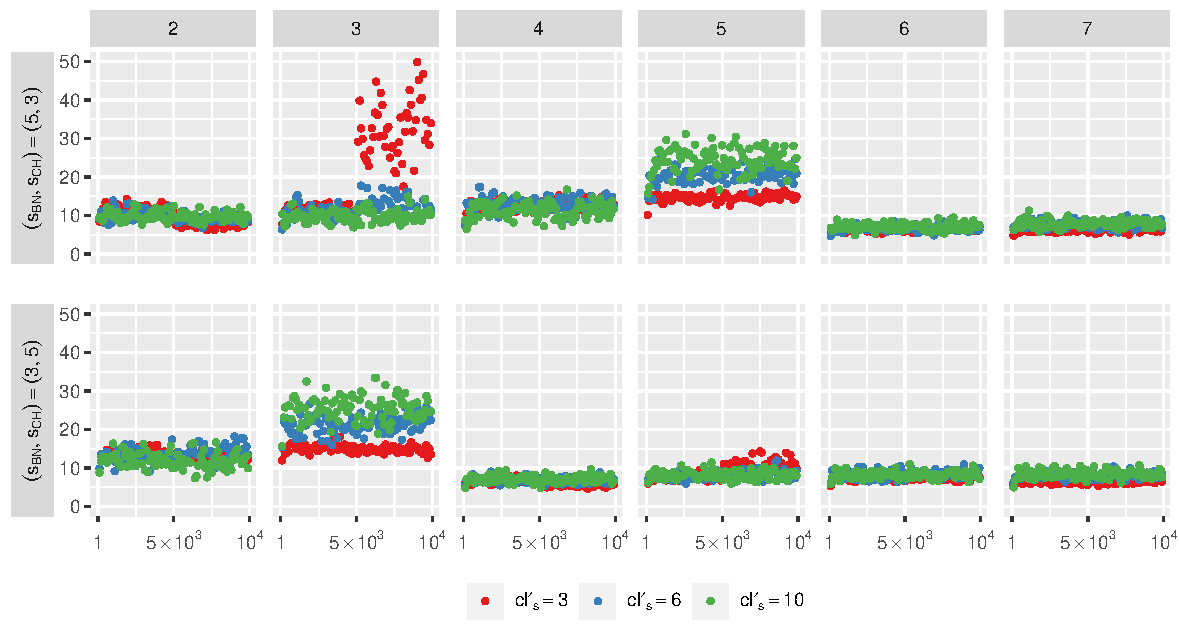
\includegraphics[width=1\textwidth]{BufferIncrease2_Waiting_time_MEAN}
\caption[Waiting time RW KPI behavior with different initial buffer capacity levels]{Waiting time RW KPI behavior considering different initial buffer capacity levels $cl_s'$ and two bottleneck-changing stage configurations $(s_{BN},s_{CH})$. Models with $cl_s''=20$.}
\label{fig:Waiting time RW KPI behavior with different initial buffer capacity levels}
\end{figure}
Figure \ref{fig:Waiting time RW KPI behavior with different initial buffer capacity levels} shows average Waiting\_time behavior considering different initial buffer capacities $cl_s'$. \\When a capacity limit increases:
\begin{itemize}
\item If buffers tend to be saturated, average Waiting\_time significantly changes. \\This is visible in models with before-change buffer capacity $cl_s'=3$, in particular in correspondence with the changing stage $s_{CH}$.
\item If buffers tend to be unsaturated, average Waiting\_time does not change. \\This is visible in models with before-change buffer capacity $cl_s'=10$.
\item If buffers are on average halfway saturated, average Waiting\_time behavior mostly depends on the position of the changing stage with respect to the bottleneck. \\This is visible in models with before-change buffer capacity $cl_s'=6$: when $s_{CH}$ is upstream $s_{BN}$ (i.e. model with configuration $(s_{BN},s_{CH})=(5,3)$), average Waiting\_time (slightly) changes in correspondence of $s_{CH}$.\footnote{This also verifies when the variation occurs in correspondence with the changing stage $s_{CH}$} When $s_{CH}$ is downstream $s_{BN}$ (i.e. model with configuration $(s_{BN},s_{CH})=(3,5)$), average Waiting\_time does not significantly change of $s_{CH}$
\end{itemize}
\subsubsection{Buffer capacity decrease effects on Waiting\_time KPI}
\begin{figure}[h]
\centering
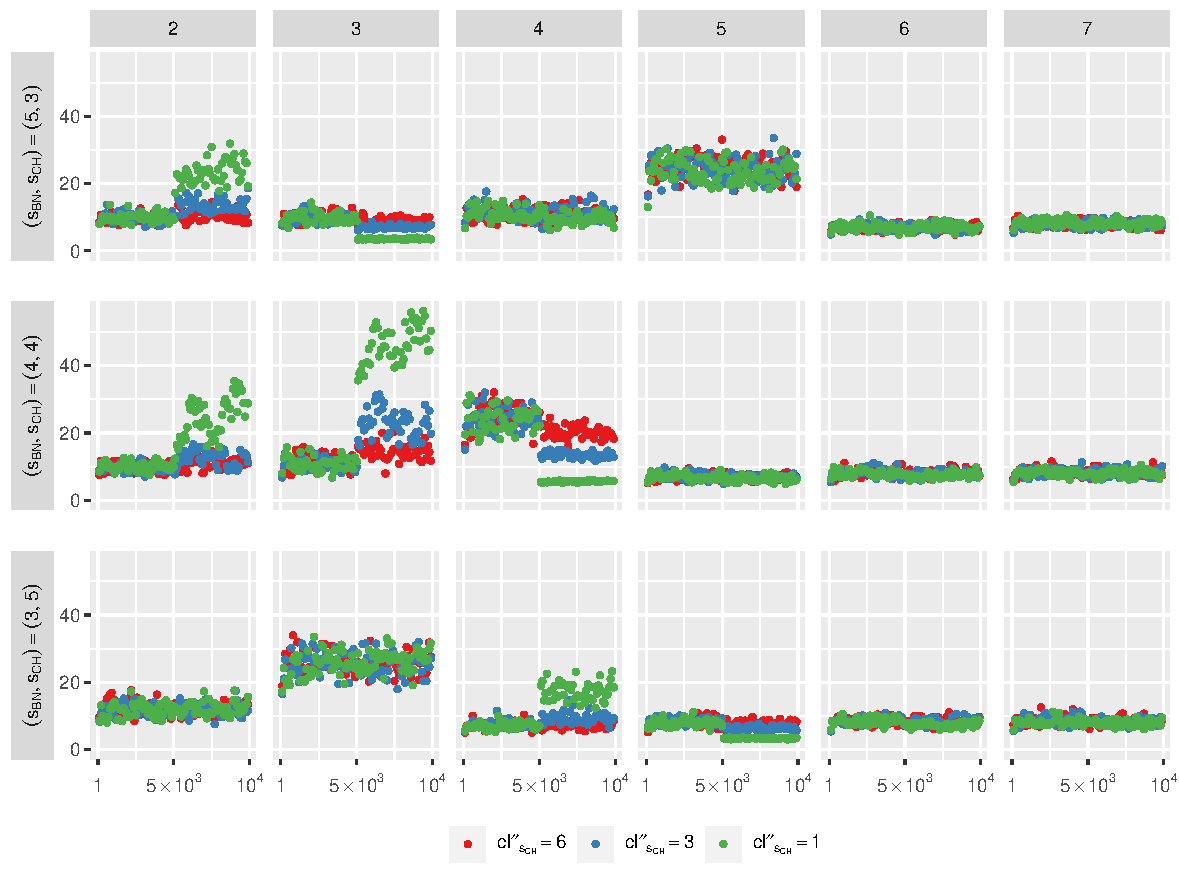
\includegraphics[width=1\textwidth]{BufferIncrease3_Waiting_time_MEAN}
\caption[Waiting time RW KPI behavior with different buffer capacity decrease levels]{Waiting time RW KPI behavior considering different buffer capacity decrease levels  $cl_s''$. Models with $cl_s'=10$)}
\label{fig:Waiting time RW KPI behavior with different buffer capacity decrease levels}
\end{figure}
Figure \ref{fig:Waiting time RW KPI behavior with different buffer capacity decrease levels} shows average Waiting\_time behavior when a buffer capacity decreases.
\begin{itemize}
\item If a buffer capacity reduces 
\begin{itemize}
\item In stages upstream the changing stage $s_{CH}$, average Waiting\_time increases.
\item In correspondence of the changing stage $s_{CH}$, average Waiting\_time decreases.
\item In stages downstream the changing stage $s_{CH}$, average Waiting\_time does not significantly change.
\end{itemize}
\item Average Waiting\_time variations are wider the larger the decrease of buffer capacity is. \\This is visible comparing models with different after-change buffer capacities $cl_{s_{CH}}''$. 
\item Average Waiting\_time variations are 
\begin{itemize}
\item wider if the changing stage is upstream or in correspondence with the bottleneck ($s_{CH} \leqslant s_{BN}$)
\item narrower if the changing stage is downstream the bottleneck ($s_{CH}>s_{BN}$)
\end{itemize}
This is visible comparing models having bottleneck-changing stage configurations $(s_{BN},s_{CH})=(5,3)$ (changing stage upstream the bottleneck) or $(s_{BN},s_{CH})=(4,4)$ (changing stage in correspondence with the bottleneck) with models having $(s_{BN},s_{CH})=(3,5)$ (changing stage downstream the bottleneck). 
\item Average Waiting\_time variations in a certain stage $s$ are less and less relevant the further stage $s$ is from the changing stage $s_{CH}$, both upstream and downstream. 
\end{itemize}
\subsubsection{Variation conceal caused by before-change high capacity buffers}
It is important to highlight that not every buffer capacity limit variation is detectable using Waiting\_time or Average\_Queue. Indeed, when before-change buffer sizes are much higher than necessary, and so underused and largely unsaturated during the process, buffer capacity growths or limited capacity reductions are impossible to notice. It verifies because, if queues in buffers are consistently much lower than the capacity limit, a variation of the limit will not have effects on the queue: in case of a capacity increase, the added room is not used, while in case of a capacity decrease (if not too large), the removed space was not used before the change and, so, jobs are not influenced by the change.
\begin{figure}[h]
\centering
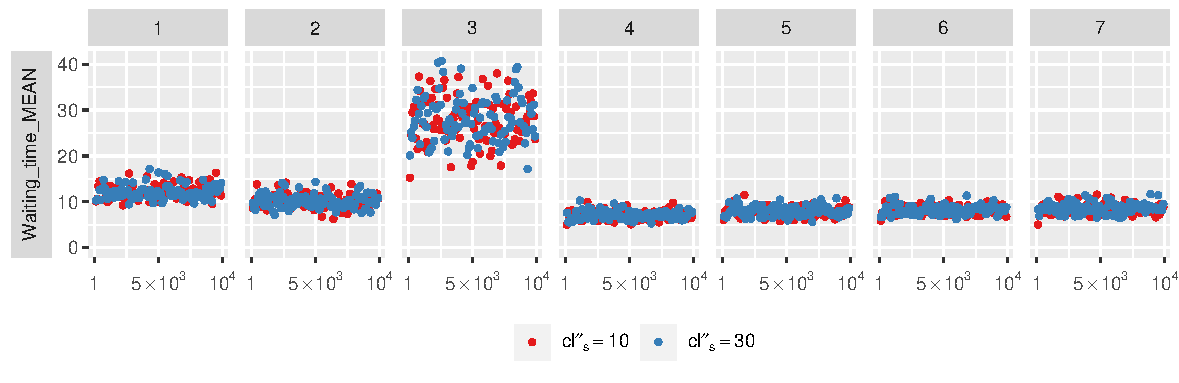
\includegraphics[width=1\textwidth]{BufferIncrease8_Waiting_time_MEAN}
\caption[Waiting time RW KPI behavior with different buffer capacity variation levels and high before-change buffer capacity limits]{Waiting time RW KPI behavior considering different buffer capacity variation levels $cl_s''$. Models with configuration $(s_{BN},s_{CH})=(3,5)$ and $cl_s'=20$.}
\label{fig:Waiting time RW KPI behavior with different buffer capacity variation levels and high before-change buffer capacity limits}
\end{figure}
Figure \ref{fig:Waiting time RW KPI behavior with different buffer capacity variation levels and high before-change buffer capacity limits} helps to visualize this kind of situation: all the buffers have high capacities ($cl_s'=20$), and so are extremely unsaturated. When the changing stage capacity limit increases to $cl_{s_{5}}=30$, average Waiting\_time behavior does not change. Moreover, since the changing stage is downstream the bottleneck ($s_{CH}=5>s_{BN}=3$), even a capacity limit decrease has no visible effects on average Waiting\_time.\\
Before-change high capacity buffers have also the same effects on Blocking\_time and Starving\_time KPIs, which are discussed in the next chapter. Therefore, it is possible to conclude that, if a buffer capacity change occurs in correspondence with a high capacity and extremely unsaturated buffer, it is not detectable with any KPI defined in this thesis. 
\newpage
\subsection{Blocking\_time and Starving\_time KPIs}
\label{Blocking time and Starving time KPIs - Buffer capacity variation}
Since Blocking\_time and Starving\_time KPI behaviors are specular (as seen in subsection \ref{Blocking time, Starving time and respective Stage State KPIs - Processing time variation}), they are analyzed together in this subsection. These KPI behaviors are influenced by both the production capacities of resources and the capacities of buffers. 
\subsubsection{Buffer capacity increase effects on Blocking\_time and Starving\_time KPIs}
\begin{figure}[h] 
\centering
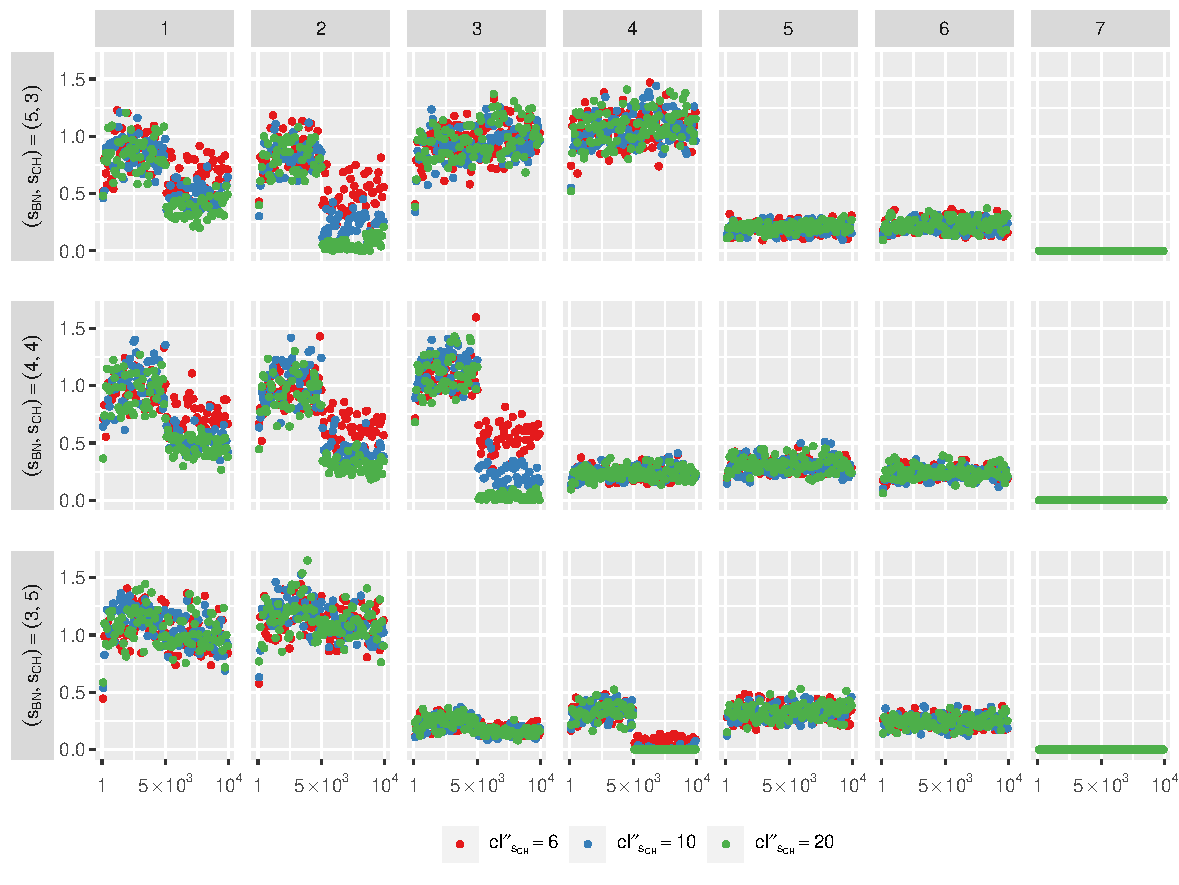
\includegraphics[width=1\textwidth]{BufferIncrease4_Blocking_time_MEAN}
\caption[Blocking time RW KPI behavior with different buffer capacity increase levels]{Blocking time RW KPI behavior considering different buffer capacity increase levels $cl_{s_{CH}}''$ and three bottleneck - changing stage configurations $(s_{BN},s_{CH})$. Models with $cl_s'=3$.}
\label{fig:Blocking time RW KPI behavior with different buffer capacity increase levels}
\end{figure}
\begin{figure}[h] 
\centering
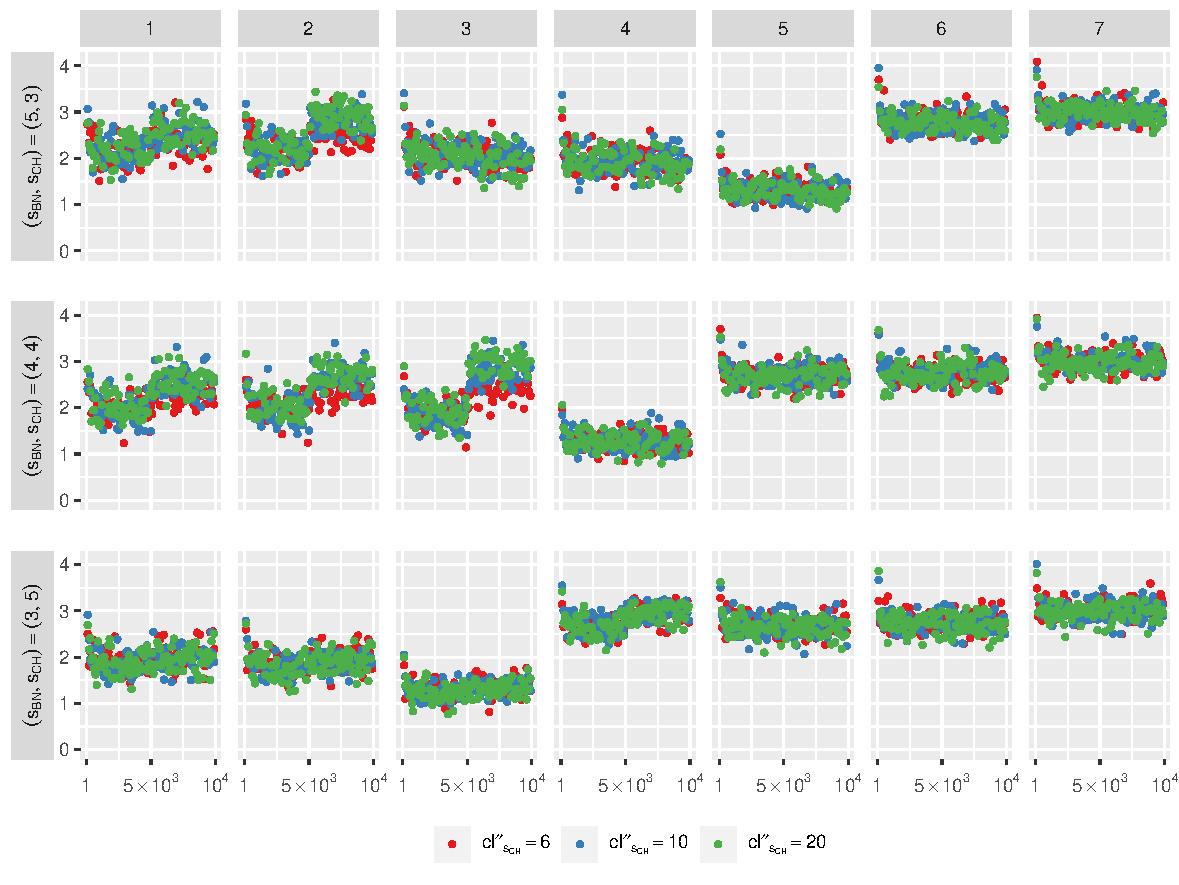
\includegraphics[width=1\textwidth]{BufferIncrease5_Starving_time_MEAN}
\caption[Starving time RW KPI behavior with different buffer capacity decrease levels]{Starving time RW KPI behavior considering different buffer capacity increase levels $cl_{s_{CH}}''$ and three bottleneck - changing stage configurations $(s_{BN},s_{CH})$. Models with $cl_s'=3$.}
\label{fig:Starving time RW KPI behavior with different buffer capacity increase levels}
\end{figure}
Figure \ref{fig:Blocking time RW KPI behavior with different buffer capacity increase levels} and figure \ref{fig:Starving time RW KPI behavior with different buffer capacity increase levels} show, respectively, average Blocking\_time and average Starving\_time behaviors in case of buffer capacity increases. 
\begin{itemize}
\item If a buffer capacity increases
\begin{itemize}
\item In stages upstream the changing stage $s_{CH}$, average Blocking\_time decreases and average Starving\_time increases.
\item In correspondence of the changing stage $s_{CH}$, average Blocking\_time increases and average Starving\_time decreases.
\item In stages downstream the changing stage $s_{CH}$, both average Blocking\_time and average Starving\_time do not significantly change.
\end{itemize}
\item Average Blocking\_time and average Starving\_time variations are wider the larger the increase of buffer capacity is. \\This is visible comparing models with different after-change buffer capacities $cl_{s_{CH}}''$. 
\item Average Blocking\_time and average Starving\_time variations are 
\begin{itemize}
\item wider if the changing stage is upstream or in correspondence with the bottleneck ($s_{CH} \leqslant s_{BN}$)
\item narrower if the changing stage is downstream the bottleneck ($s_{CH}>s_{BN}$)
\end{itemize}
This is visible comparing models having bottleneck-changing stage configurations $(s_{BN},s_{CH})=(5,3)$ (changing stage upstream the bottleneck) or $(s_{BN},s_{CH})=(4,4)$ (changing stage in correspondence with the bottleneck) with models having $(s_{BN},s_{CH})=(3,5)$ (changing stage downstream the bottleneck) . 
\item Average Blocking\_time and average Starving\_time variations in a certain stage $s$ are less and less relevant the further stage $s$ is from the changing stage $s_{CH}$, both upstream and downstream $s_{CH}$. 
\end{itemize}
\subsubsection{Blocking\_time and Starving\_time behaviors considering different initial buffer sizes $cl_s'$}
As for Waiting\_time, buffer capacity variations may have no effects on Blocking\_time and Starving\_time. The occurrence of a change of these KPIs mainly rely on the initial buffer saturation levels before the capacity variation verifies. 
\begin{figure}[h] 
\centering
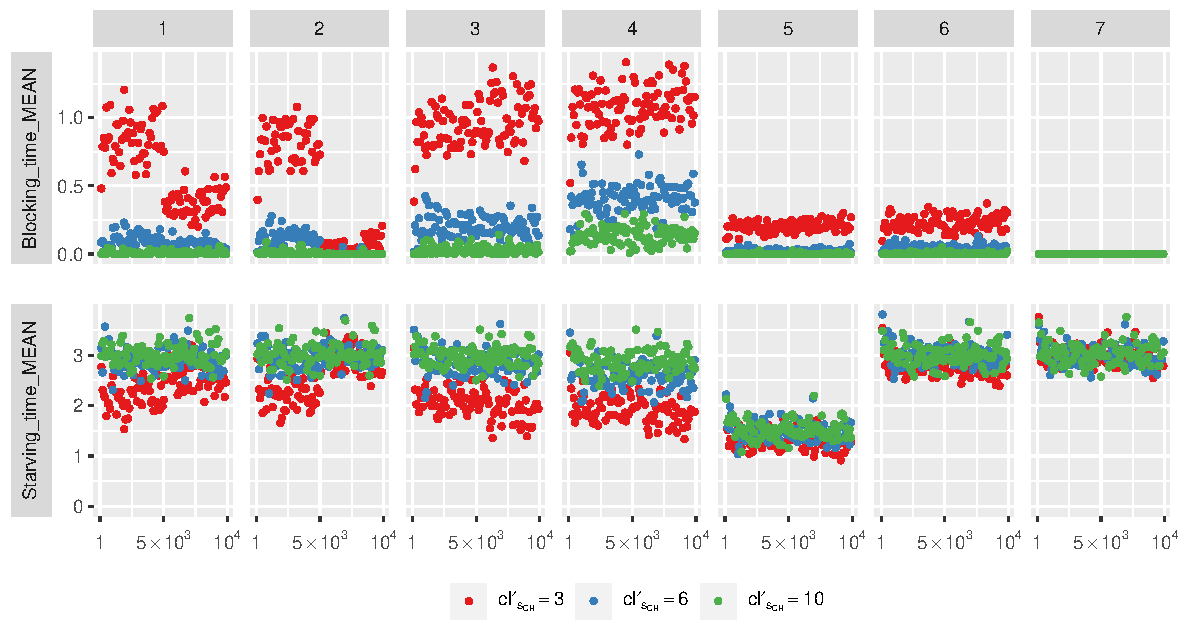
\includegraphics[width=1\textwidth]{BufferIncrease6_Blocking_time_MEAN_Starving_time_MEAN}
\caption[Blocking time and Starving time RW KPIs behaviors with different initial buffer capacity levels]{Blocking time and Starving time RW KPIs behaviors considering different initial buffer capacity levels $cl_s'$. Models with configuration $(s_{BN},s_{CH})=(5,3)$ and after-change value $cl_s''=20$.}
\label{fig:Blocking time and Starving time RW KPIs behaviors with different initial buffer capacity levels}
\end{figure}
Figure \ref{fig:Waiting time RW KPI behavior with different initial buffer capacity levels} shows average Blocking\_time and Starving\_time behaviors considering different initial buffer capacities $cl_s'$. \\When a capacity limit increases:
\begin{itemize}
\item If buffers tend to be saturated, average Blocking\_time and Starving\_time significantly change. \\This is visible in models with before-change buffer capacity $cl_s'=3$, in particular in correspondence with the changing stage $s_{CH}=3$.
\item If buffers tend to be unsaturated, average Blocking\_time and Starving\_time do not change. \\This is visible in models with before-change buffer capacity $cl_s'=10$.
\item If buffers are on average halfway saturated, average Blocking\_time and Starving\_time behaviors mostly depend on the position of the changing stage with respect to the bottleneck. \\This is visible in models with before-change buffer capacity $cl_s'=6$: when $s_{CH}$ is upstream $s_{BN}$ (i.e. model with configuration $(s_{BN},s_{CH})=(5,3)$), average Blocking\_time and Starving\_time (slightly) change in correspondence and upstream $s_{CH}$. When $s_{CH}$ is downstream $s_{BN}$ (i.e. model with configuration $(s_{BN},s_{CH})=(3,5)$), average Blocking\_time and Starving\_time do not significantly change.
\end{itemize}
\subsubsection{Buffer capacity decrease effects on Blocking\_time and Starving\_time}
\begin{figure}[h] 
\centering
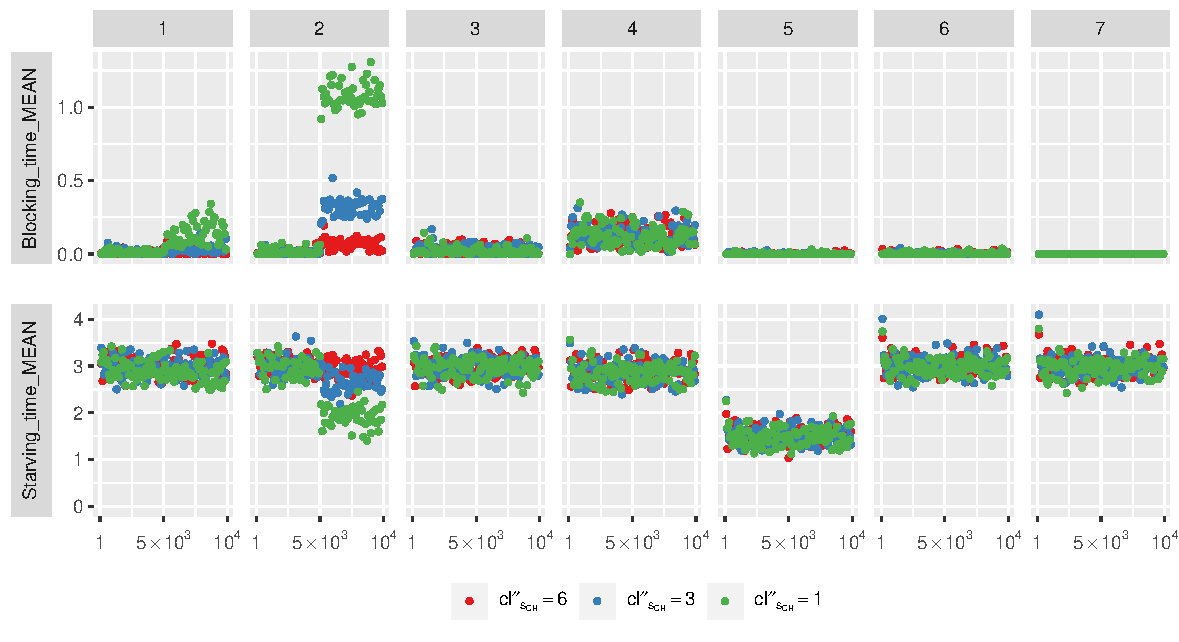
\includegraphics[width=1\textwidth]{BufferIncrease7_Blocking_time_MEAN_Starving_time_MEAN}
\caption[Blocking time and Starving time RW KPIs behaviors with different buffer capacity decrease levels]{Blocking time and Starving time RW KPIs behaviors considering different buffer capacity decrease levels $cl_s''$. Models with configuration $(s_{BN},s_{CH})=(5,3)$ and $cl_s'=10$.}
\label{fig:Blocking time and Starving time RW KPIs behaviors with different buffer capacity decrease levels}
\end{figure}
Figure \ref{fig:Waiting time RW KPI behavior with different buffer capacity decrease levels} shows average Blocking\_time and Starving\_time behaviors when a buffer capacity decreases.
\begin{itemize}
\item If a buffer capacity reduces 
\begin{itemize}
\item In stages upstream the changing stage $s_{CH}$, average Blocking\_time increases and average Starving\_time decreases.
\item In correspondence of the changing stage $s_{CH}$, average Blocking\_time decreases and average Starving\_time increases.
\item In stages downstream the changing stage $s_{CH}$, both average Blocking\_time and average Starving\_time do not significantly change.
\end{itemize}
\item Average Blocking\_time and Starving\_time variations are wider the larger the decrease of buffer capacity is. \\This is visible comparing models with different after-change buffer capacities $cl_{s_{CH}}''$. 
\item Average  Blocking\_time and Starving\_time variations are 
\begin{itemize}
\item wider if the changing stage is upstream or in correspondence with the bottleneck ($s_{CH} \leqslant s_{BN}$)
\item narrower if the changing stage is downstream the bottleneck ($s_{CH}>s_{BN}$)
\end{itemize}
\item Average  Blocking\_time and Starving\_time variations in a certain stage $s$ are less and less relevant the further stage $s$ is from the changing stage $s_{CH}$, both upstream and downstream. 
\end{itemize}